%%%%%%%%%%%%%%%%%%%%%%%%%%%% Huong dan su dung compiler %%%%%%%%%%%%%%%%%%%%%%%%
% Latex>biber>latex>makeglossary>latex> makeindex > latex > pdflatex > view-pdf%
%%%%%%%%%%%%%%%%%%%%%%%%%%%%%%%%%%%%%%%%%%%%%%%%%%%%%%%%%%%%%%%%%%%%%%%%%%%%%%%%

\documentclass[12pt,a4paper,reqno, oneside]{book}
\makeindex
\usepackage[utf8]{vietnam}
\usepackage{amsmath, amsthm, amssymb,latexsym,amscd,amsfonts,enumerate}
\usepackage[style=abntex2-alf,backend=biber,style=numeric,sorting=ynt,hyperref=auto,doi=true]{biblatex}
\addbibresource{thesis.bib}
\usepackage{stdclsdv}
\usepackage[]{tocbibind}
\usepackage[titletoc]{appendix}
\usepackage[hidelinks]{hyperref}
\usepackage{indentfirst}
%%%%%%%%%%%%%%%%%%%%%%%%%%%%%%%% trang tri %%%%%%%%%%%%%%%%%%%%%%%%%%%%%%%%%%%%%
\setlength{\oddsidemargin}{0in}
\setlength{\textwidth}{6.in}
\setlength{\topmargin}{-0.5in}
\setlength{\textheight}{9.25in}
\renewcommand{\baselinestretch}{1.5}
\usepackage{multicol, color, fancyhdr, graphicx, wrapfig}
\usepackage{epstopdf}

\pagenumbering{roman}\pagestyle{plain}
\pagestyle{fancy}
\lhead{\it Tương tác lực giữa phân tử VP35 và dsRNA của virus Ebola}
\rhead{\it }
\lfoot{\it Nguyễn Hữu Quý Ngân} 			         
\rfoot{\it Theoretical Physics - HCMUS}
\renewcommand{\headrulewidth}{1,2pt} 			
\renewcommand{\footrulewidth}{1,2pt}   % Cái này là tiêu đề chạy

%%%%%%%%%%%%%%%%%%%%%%%%%%%% Figures and Table %%%%%%%%%%%%%%%%%%%%%%%%%%%%%%%%%
\usepackage{afterpage, caption, subcaption}
\usepackage{tikz} %Thư viện shape
\usetikzlibrary{shapes.geometric, arrows,positioning} % Flow chart

%%%%%%%%%%%%%%%%%%%%%%%%%%%% Tu dien viet tat %%%%%%%%%%%%%%%%%%%%%%%%%%%%%%%%%%

\usepackage{glossaries}
\makeglossaries
\setacronymstyle{long-short}
\newacronym{ebov}{EBOV}{virus Ebola}
\newacronym{zebov}{ZEBOV}{Zaire Ebola}
\newacronym{evd}{EVD}{Bệnh Ebola - Ebola Virus Disease -}
\newglossaryentry{ligand}
{
name={phối tử},
description={ligand là một (hoặc một nhóm) phân tử có khả năng gắn vào một nhóm phân tử khác để tạo nên phức hợp với chức năng riêng biệt.}}
\newglossaryentry{receptor}
{
name={thụ thể},
description={receptor là phân tử nằm ở màng tế bào có chức năng thu nhận tín hiệu hóa học cho tế bào đó.}}
\newglossaryentry{R312A}
{
name={Arg312Ala},
description={Đột biến amino acid Arginine ở vị trí thứ 312 thành Alanine.}}
\newglossaryentry{K339A}
{
name={Lys339Ala},
description={Đột biến amino acid Lysine ở vị trí thứ 339 thành Alanine.}}
\newglossaryentry{K282A}
{
name={Lys282Ala},
description={Đột biến amino acid Lysine ở vị trí thứ 282 thành Alanine.}}
\newacronym{ehf}{EHF}{Sốt xuất huyết Ebola - Ebola Hemmohaegic Fever -}
\newacronym{md}{MD}{phương pháp động học phân tử - Molecular dynamics -}
\newacronym{smd}{SMD}{Steered Molecular Dynamics}
\newacronym{dsrna}{dsRNA}{chuỗi kép RNA - double-strain RNA -}
\newacronym{iid}{IID}{Interferon Inhibitor Domain}
\newacronym{meta}{metadynamics}{metadynamcis}
\newacronym{amber}{amber99sb ff}{trường lực AMBER99SB}
\newacronym{gp}{GP}{Glycoprotein}
\newglossaryentry{ifn}
{
name={IFN},
description={Interferon (IFN) là một nhóm các protein tự nhiên được sản xuất bởi các tế bào của hệ miễn dịch ở hầu hết các động vật nhằm chống lại các tác nhân ngoại lai như virus, vi khuẩn, kí sinh trùng và tế bào ung thư.\cite{DeAndrea2002}},
%other options
}
\newacronym{np}{NP}{Nucleoprotein}
\newglossaryentry{rig-i}
{
name={RIG-I},
description={retinoic acid-inducible gene 1 là một loại enzym có chức năng phát hiện chuỗi vật chất di truyền của các virus cúm A, virus Sendai, họ flavivirus (virus sốt xuất huyết, viêm não Nhật Bản,...). Tuy nhiên RIG-I không phát hiện được retrovirus hay virus có vật chất di truyền là DNA.\cite{Kato2008}},
%other options
}
\newglossaryentry{residue}
{
name={vị trí amino acid},
description={mỗi amino acid tại vị trí cụ thể sẽ có một vai trò cụ thể, vì vậy cần xác định tên amino acid và số thứ tự của nó trong chuỗi protein.},
%other options
}









\begin{document}

\newpage
\begin{titlepage}
\centerline{\bf ĐẠI HỌC QUỐC GIA TP.HCM}
\centerline{\bf TRƯỜNG ĐẠI HỌC KHOA HỌC TỰ NHIÊN}
\centerline{\bf KHOA VẬT LÝ-VẬT LÝ KỸ THUẬT}
\vspace*{1cm}
\centerline{KHÓA LUẬN TỐT NGHIỆP}
\centerline{Chuyên ngành: Vật lý Lý thuyết}
\vspace*{1cm}
\centerline{\bf Nguyễn Hữu Quý Ngân}
\vspace*{3cm}
\centerline{\Large\bf KHẢO SÁT TƯƠNG TÁC GIỮA PHÂN TỬ PROTEIN VP35}
\vspace*{0.5cm}
\centerline{\Large\bf VÀ dsRNA CỦA VIRUS EBOLA}
\vspace*{4cm}
\centerline{\bf Người hướng dẫn: }
\centerline{\bf TS. Nguyễn Hà Hùng Chương}
\vfill
\centerline{\bf TP.HCM 07/2015}
\end{titlepage}

\pagestyle{plain}
%\input Loicamon

\cleardoublepage% \clearpage
\pagestyle{fancy}
\pagenumbering{roman}
\tableofcontents
\clearpage

%%%%%%%%%%%%%%%%%%%                      %%%%%%%%%%%%%%%%%%%%%%%%
%%%%%%%%%%%%%%%%%%%      Loi cam on      %%%%%%%%%%%%%%%%%%%%%%%%
%%%%%%%%%%%%%%%%%%%                      %%%%%%%%%%%%%%%%%%%%%%%%
\newpage
\addcontentsline{toc}{chapter}{\protect{}Lời cảm ơn}
\chapter*{Lời cảm ơn}
Đề tài hoàn thành được là nhờ sự hỗ trợ rất lớn từ quý thầy, các anh chị và các bạn trong nhóm nghiên cứu.

Em xin cảm ơn TS. Nguyễn Hà Hùng Chương rất nhiều vì thầy đã luôn dành thời gian và kinh nghiệm để hỗ trợ em hết mình trong việc giải quyết các khó khăn. Em xin cảm ơn TS. Võ Thành Văn đã nỗ lực truyền đạt kiến thức cho tập thể lớp, đồng thời tạo cho em nếp suy nghĩ logic và kỹ năng tính toán cần có. Em xin cảm ơn TS. Vũ Quang Tuyên đã luôn lắng nghe và hỗ trợ em cùng các bạn trong lớp. Em xin cảm ơn TS. Võ Quốc Phong vì đã chia sẻ những ý kiến thiết thực về nhân cách sống. Em xin cảm ơn TS. Nguyễn Hữu Nhã đã tận tình hỗ trợ và tìm mọi cách để tạo điều kiện học tập tốt nhất cho sinh viên bộ môn.

Em xin cảm ơn anh Nguyễn Quý Trường và anh Trần Phước Duy đã luôn dành thời gian giúp đỡ em về mặt kỹ thuật. Em xin cảm ơn anh Minh Trung, anh Minh Nhật, anh Anh Tuấn đã cung cấp cho em bản khoá luận, giúp em thừa kế kiến thức các anh đã bỏ công nghiên cứu.

Xin cảm ơn các bạn lớp Vật lý lý thuyết khoá 2011. Các bạn đã luôn hỗ trợ lẫn nhau hết mình.

Trên hết, con xin cảm ơn ba mẹ đã luôn tin tưởng con có thể học và theo đuổi nghiên cứu khoa học. Em xin cảm ơn chị gái đã luôn tin tưởng và giúp đỡ em. Xin cảm ơn em gái đã chăm sóc anh trong suốt thời gian làm việc căng thẳng.

\printglossaries
\addcontentsline{toc}{chapter}{Từ điển chú giải}
\clearpage

\newpage
\pagestyle{fancy}
\listoffigures



%\newpage
%\pagestyle{fancy}

%%%%%%%%%%%%%%%%%%%     Loi mo dau       %%%%%%%%%%%%%%%%%%%%%%%%
%%%%%%%%%%%%%%%%%%%                      %%%%%%%%%%%%%%%%%%%%%%%%
\newpage
\addcontentsline{toc}{chapter}{\protect{}Lời mở đầu}
\chapter*{Lời mở đầu}
	Ebola là bệnh sốt xuất huyết có tỷ lệ tử vong cao và chưa có thuốc đặc trị cũng như vaccine để phòng ngừa. Để có thể tìm được thuốc, chúng ta cần tìm hiểu các protein tham gia vào quá trình virus Ebola sao chép. Một trong những protein có nhiều vai trò trong quá trình sao chép của virus Ebola là VP35. Một trong các chức năng của VP35 là gắn vào vật chất di truyền của virus Ebola (\gls{dsrna}) và ngăn cản hệ thống miễn dịch phát hiện ra sự có mặt của \gls{dsrna} trong tế bào.
	
	Đề tài tập trung vào việc phân tích tương tác của phân tử VP35 và \gls{dsrna} của virus Ebola (\gls{ebov}) nhằm đánh giá các amino acid có vai trò quan trọng trong tương tác giữa hai phân tử trên. Đề tài sử dụng phương pháp mô phỏng \gls{smd}, nhằm khảo sát sự chuyển trạng thái từ VP35--\gls{dsrna} tương tác với nhau sang trạng thái VP35--\gls{dsrna} không tương tác. Kết quả của khóa luận cho thấy các amino acid Arg312 và Lys339 của VP35 đóng vai trò quan trọng trong tương tác VP35-dsRNA, kết quả này phù hợp với thực nghiệm \cite{Leung2010}.
	
	Đồng thời đề tài cũng cho thấy đột biến amino acid Lys282 từ Lysine thành Alanine (Lys282Ala) làm giảm khả năng liên kết giữa VP35 và \gls{dsrna}. Do vậy Lys282 được dự đoán là đóng vai trò quan trọng trong tương tác giữa VP35 và \gls{dsrna}.
	
%	Phương pháp được sử dụng là \gls{smd}. Mô hình phân tử nước được sử dụng là TIP-4P\cite{Horn2004} và \gls{amber}\cite{Hornak2006} trong quá trình mô phỏng động học.
	
	Đề tài gồm 4 chương:
	\begin{itemize}
	\item Chương 1: Bệnh Ebola, \gls{ebov} và sự cần thiết của việc nghiên cứu \gls{ebov}, quá trình \gls{ebov} sao chép và vai trò của protein VP35, một số phương án ngăn chặn \gls{ebov} và một số nghiên cứu gần đây.
	\item Chương 2: Các cấu hình của VP35 được khảo sát, \gls{md} và phần mềm, công cụ sử dụng để khảo sát tương tác giữa VP35 và \gls{dsrna}.
	\item Chương 3: Trình bày các kết quả thu được và thảo luận tương ứng.
	\item Chương 4: Các kết luận và hướng phát triển tiếp theo của đề tài.
	\end{itemize}

	%Do thời gian thực hiện khóa luận không nhiều, kiến thức còn hạn chế nên đề tài không tránh khỏi sai sót. Tác giả rất mong nhận được sự góp ý và những ý kiến phản biện của quý thầy cô và các bạn.
	\textrm{Xin chân thành cảm ơn!}
 
 
 
 
%%%%%%%%%%%%%%%%%%%     Chuong 1       %%%%%%%%%%%%%%%%%%%%%%%%
%%%%%%%%%%%%%%%%%%%                    %%%%%%%%%%%%%%%%%%%%%%%%
\newpage
\pagestyle{fancy}
\setcounter{page}{1}
\pagenumbering{arabic}
\setcounter{chapter}{0}
\chapter{Tổng quan}

\section{Bệnh do Virus Ebola}

	\gls{evd} hay \gls{ehf} là bệnh truyền nhiễm trên động vật có vú gây bởi \glsentryfull{ebov}. Bệnh được phát hiện lần đầu năm 1976 tại Trung Phi\cite{Feldmann2003}. Tỉ lệ tử vong nếu không được chữa trị lên đến 90\% ở chủng \gls{zebov}. Đây là bệnh có tốc độ bùng phát cao và khó kiểm soát do Ebola có thể lây truyền qua nhiều động vật là vật chủ trung gian, đồng thời lây truyền qua tiếp xúc với dịch tiết từ cơ thể người bệnh\cite{Colebunders2000}.
	
	\gls{evd} đặc biệt nguy hiểm và có khả năng xuất hiện ở các nước có khí hậu nhiệt đới, cận nhiệt\cite{Ansari2014}. Đồng thời, \gls{evd} lây truyền qua dơi ăn trái cây và các động vật như tinh tinh, khỉ, heo\cite{Kuhn2010}, nên khả năng xuất hiện ở Việt Nam là rất cao. Trong nhiều thập kỷ, việc tìm hiểu về \gls{ebov} được quan tâm nhiều khi vũ khí sinh học trở nên phát triển\cite{Feldmann2003, Lee2009}.
	
\subsection{Các protein của \glsentrytext{ebov}}

	Cần biết rõ về các protein có trong \gls{ebov} để phác thảo được các phương án tấn công \gls{ebov} được nói đến ở mục tiếp theo.
	\Gls{ebov} thuộc họ Filoviridae, bộ Mononegravirale, tức là \gls{ebov} thuộc họ virus có vật chất di truyền RNA gram âm và có hình sợi\cite{Kuhn2010}. \Gls{ebov} được cấu tạo bởi 7 loại protein với các chức năng khác nhau\cite{Huang2002}.
	\begin{figure}[h]
	\centering
	\begin{subfigure}{\textwidth}
	\centering
	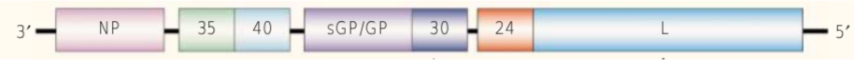
\includegraphics[width=0.7\textwidth,natwidth=610,natheight=642]{dsRNA_encode}
	\caption{Bảy loại protein được mã hoá trên RNA của \gls{ebov}}
	\label{fig:encode}
	\end{subfigure}\\
	\begin{subfigure}{\textwidth}
	\centering
	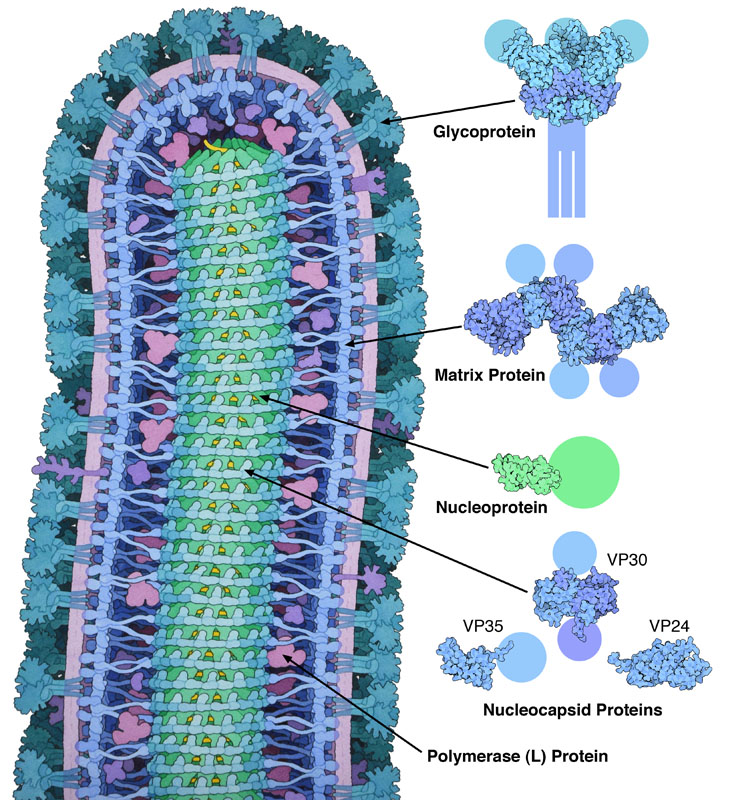
\includegraphics[width=0.7\textwidth,natwidth=610,natheight=642]{virion}
	\caption{Vị trí tương đối của các protein trong \gls{ebov}}
	\label{fig:ebola_proteins}
	\end{subfigure}
	\end{figure}
	\begin{itemize}
	\item \gls{gp} là protein nằm ở vỏ của virus, mang các thụ thể như các chìa khóa giúp \gls{ebov} đột nhập vào tế bào\cite{Johnson2006, Lee2009}.
	\item VP40 là protein ma trận, giúp định hình cấu trúc cho \gls{ebov}\cite{Dessen2000, Noda2002}.
	\item VP24 là protein có vai trò ngăn chặn các \gls{ifn} kích hoạt các gene mã hóa các protein mang tính báo động của cơ thể\cite{Reid2006}.
	\item VP30 là protein có vai trò hỗ trợ phiên mã \gls{dsrna}\cite{Weik2002}.
	\item L protein và \gls{np}\cite{Feldmann2003,Dziubanska:be5269} có vai trò quan trọng trong quá trình phiên mã \gls{dsrna}, đồng thời \gls{np} giữ cho chuỗi đơn RNA của \gls{ebov} không bị tổn hại\cite{Dziubanska:be5269}
	\item VP35 là phân tử có nhiều cấu trúc thực nghiệm và nắm giữ nhiều vai trò quan trọng trong quá trình phiên mã và vô hiệu cơ chế phát hiện RNA lạ của cơ thể người\cite{Muhlberger1999,Basler2000,Basler2003,Enterlein2006,Feng2007,Prins2009}.
	\end{itemize}

\section{Cơ chế hoạt động của EBOV}
Biết được vòng đời của \gls{ebov}, ta có thể đề ra các hướng ngăn chặn \gls{ebov}
\subsection{Quá trình xâm nhập và sao chép của EBOV}
		\begin{figure}[t!]
		\centering
		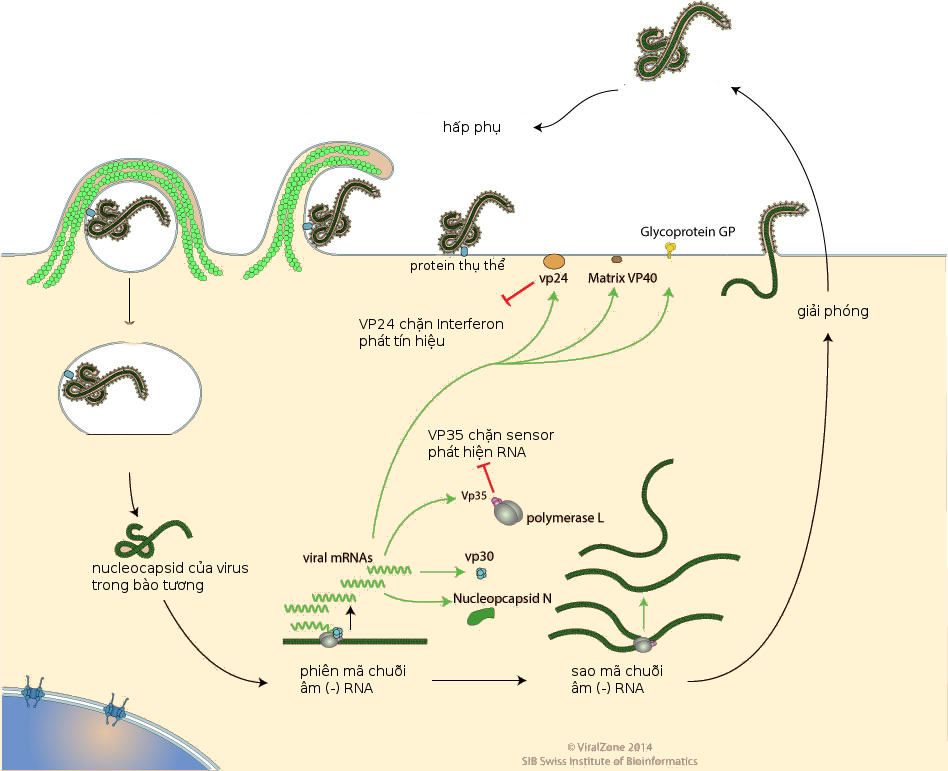
\includegraphics[width=1.0\textwidth,natwidth=610,natheight=642]{Ebolavirus_cycle.png}
		\caption{Vòng đời của \gls{ebov}. Nguồn:http://www.expasy.org/}
		\label{fig:viruscycle}
		\end{figure}

		EBOV thâm nhập tế bào thành mạch máu và thực hiện quá trình phiên mã, dịch mã, tổng hợp vật chất. Trong quá trình sao chép, protein VP35 sẽ bất hoạt phân tử \gls{rig-i} (là một loại enzym có chức năng phát hiện chuỗi vật chất di truyền của các virus cúm A, virus Sendai, họ flavivirus) và vô hiệu hóa hệ thống miễn dịch. Sau khi nhân lên với số lượng lớn, EBOV sẽ giải phóng khỏi tế bào và xâm nhập các tế bào khác\cite{Colebunders2000} (xem hình \ref{fig:viruscycle}).
\subsection{Quá trình hệ thống miễn dịch hoạt động}

		Phân tử \gls{rig-i} có vai trò phát hiện các dsRNA lạ và kích hoạt tế bào sản xuất \gls{ifn}$\alpha / \beta$\cite{Cardenas2006}. Sau khi tế bào bệnh bị phá vỡ do virus nhân lên với số lượng lớn và giải phóng ra ngoài, \gls{ifn}$\alpha / \beta$ (protein tín hiệu của tế bào bị nhiễm bệnh) cũng được giải phóng theo và bám vào thụ thể của các tế bào lân cận. Sự bám này là tín hiệu cho hệ thống miễn dịch hoạt động và phá hủy tất cả các tế bào có chứa các tác nhân lạ\cite{DeAndrea2002}.
%		\begin{figure}[h]
%		\centering
%		
%		\caption{}
%		\label{}
%		\end{figure}
\subsection{VP35 vô hiệu hệ thống miễn dịch}

		VP35 bám vào dsRNA của EBOV và không cho \gls{rig-i} phát hiện dsRNA, do \gls{rig-i} phát hiện dsRNA bằng cách liên kết với dsRNA. Theo đó, không có tín hiệu kích hoạt tế bào sản xuất IFN$\alpha / \beta$ và hệ thống miễn dịch không được báo động khi \gls{ebov} phá vỡ thành tế bào và chui ra ngoài\cite{Hartman2004}.
\subsection{Các phương án ngăn chặn EBOV}
	Bằng chứng cho thấy những trường hợp được chữa khỏi \gls{evd} có nồng độ Immunoglobulin G (IgG - kháng thể G) và Immunoglobulin T (IgT) cao. Thí nghiệm sử dụng kháng thể trên cơ thể ngựa và chuột đã thành công\cite{Feldmann2003}.
	
	Vaccine tiềm năng nhất được phát triển và đưa vào thử nghiệm là VSV-ZEBOV. Bằng cách cấy đoạn RNA mã hoá \gls{gp} của \gls{ebov} vào vesicular somatitis virus (một loại virus cùng họ với virus dại), \gls{gp} của \gls{ebov} sẽ được tổng hợp khi vesicular somatitis virus được đưa vào cơ thể và hệ miễn dịch sẽ dễ dàng nhận diện phân tử \gls{gp} do các phân tử khác của \gls{ebov} không được tổng hợp để vô hiệu hệ thống miễn dịch. Vaccine này đã được thử nghiệm thành công đối với động vật có vú\cite{Mire2015}.
	
	Ngoài ra, việc điều chế thuốc có tác dụng đặc hiệu lên các protein của \gls{ebov} cũng là một phương pháp tiềm năng. Các \gls{gp} của \gls{ebov} đôi khi chịu đột biến và các vaccine hoạt động dựa trên việc tổng hợp \gls{gp} sẽ không còn hiệu quả. Phân tử VP35 là một trong những phân tử có tính bảo tồn cao của họ Filoviridae nên nếu có thể tìm được phân tử thuốc bất hoạt được VP35 thì phân tử thuốc này sẽ có khả năng bất hoạt nhiều chủng virus thuộc họ Filoviridae.
\section{Các nghiên cứu trên thế giới về VP35}
	\begin{figure}[t!]
	\centering
	%\begin{subfigure}
	\includegraphics[width=0.7\textwidth,natwidth=610,natheight=642]{tongquan/1DK_3L25}
	\caption{Vị trí tương đối của ligand 1DK so với VP35 (màu xanh da trời) và dsRNA (màu vàng) đã được công bố trên \cite{Brown2014}.}
	\label{fig:1dk_3l25}
	%\end{subfigure}
	\end{figure}
	Ngân hàng protein thế giới (Protein Data Bank) lưu trữ các cấu trúc thực nghiệm của VP35. Trong các cấu trúc thực nghiệm thu được, có một cấu trúc của phân tử VP35 chủng Zaire Ebola (\gls{zebov}) nguyên thuỷ gắn với \gls{dsrna} của chính virus này\cite{Leung2010}. Đồng thời, việc đột biến các \gls{residue} thứ 309, 312, 339 đã được xác nhận là làm mất hoàn toàn chức năng gắn vào \gls{dsrna} của VP35\cite{Cardenas2006,Hartman2004}.
	
	Có 9 phân tử nhỏ (ligand) đã được tiên đoán là có khả năng tương tác tốt với VP35 và có tiềm năng trở thành thuốc đặc trị\cite{Brown2014,Dapiaggi2015}. Xem hình \ref{fig:1dk_3l25}. 9 phân tử này có PDBID lần lượt là: 1DK, 12G, 1DL, 11Y, 1D5, 1D6, 1D8, 1D9, 1DE. Các phân tử này can thiệp vào vùng tương tác với nucleoprotein (NP) của \gls{ebov} và gây cản trở quá trình nhân lên của virus trong điều kiện phòng thí nghiệm (\emph{in vitro}).
	
	

%%%%%%%%%%%%%%%%%%%%%%%%%%%%%%%%%%%%%%%%%%%
%+ Ket thuc Chuong 1.
%%%%%%%%%%%%%%%%%%%%%%%%%%%%%%%%%%%%%%%%%%%


\newpage
\pagestyle{fancy}
%%%%%%%%%%%%%%%%%%%     Chuong 2       %%%%%%%%%%%%%%%%%%%%%%%%
%%%%%%%%%%%%%%%%%%%                    %%%%%%%%%%%%%%%%%%%%%%%%
\setcounter{chapter}{1}
\chapter{Đối tượng và phương pháp nghiên cứu}

	Khóa luận tập trung nghiên cứu cấu hình có PDBID là 3L25 của phân tử VP35, sử dụng phương pháp \gls{smd} để đánh giá tương tác giữa VP35 và dsRNA. Đây là cấu trúc thực nghiệm duy nhất của VP35 không đột biến gắn với \gls{dsrna}.
\section{Cấu hình của VP35}
	\subsection{Cấu hình 3L25}
	
		Gồm chuỗi \gls{dsrna} dài 8 đơn vị (8bps) liên kết với 4 phân tử VP35 (chuỗi A, B, C và D). Chuỗi A và B tạo thành một nhóm, với chuỗi B gắn với đầu chuỗi dsRNA và chuỗi A gắn với dsRNA dọc theo chiều dài chuỗi. Tương tự với chuỗi C và D. Chuỗi A và C hình thành tương tác Van der Waals với dsRNA. Chuỗi B và D xuất hiện liên kết nhánh phụ trực tiếp với nhóm phosphodiester của dsRNA\cite{Leung2010} (Xem \ref{fig:vp35}).
%		\clearpage
		\begin{figure}[t!]
		\centering
		\begin{subfigure}{0.5\textheight}
		\centering
		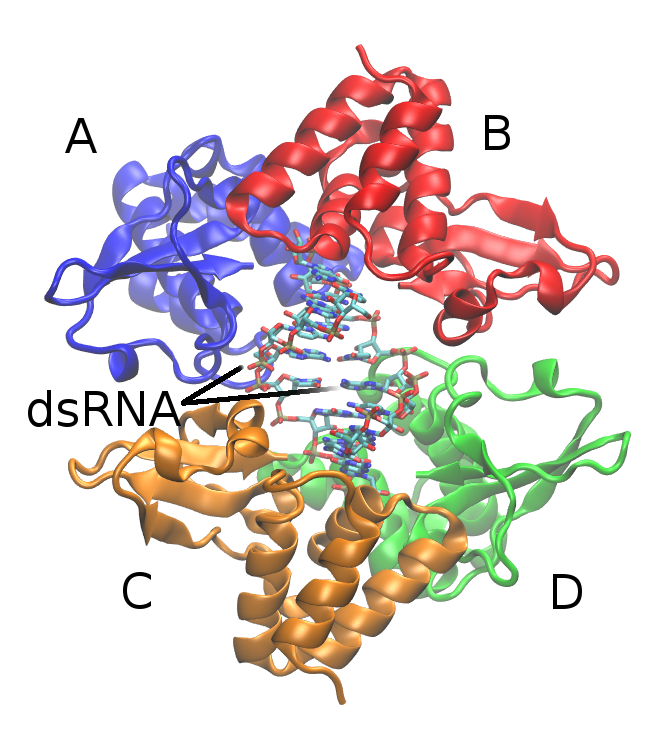
\includegraphics[width=0.7\textwidth,natwidth=610,natheight=642]{VP35.png}
		\caption{4 đơn vị phân tử VP35 bám vào \gls{dsrna} được tô màu xanh dương, đỏ, cam, xanh lá cây.}
		\label{fig:vp35}
		\end{subfigure}\\
		\begin{subfigure}{0.5\textheight}
		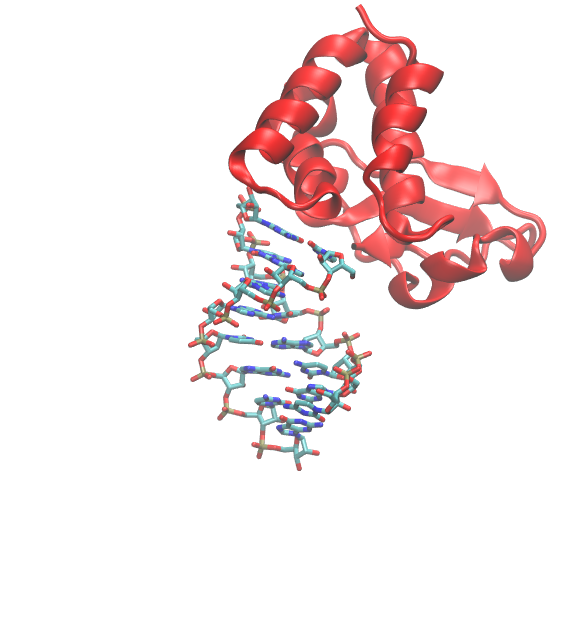
\includegraphics[width=0.9\linewidth,natwidth=610,natheight=642]{VP35_B.png}
		\vspace{-50pt}
		\caption{Chuỗi VP35 B bám vào \gls{dsrna} dài 8bps được tô màu đỏ.}
		\label{fig:vp35b}
		\end{subfigure}
		\caption{Cấu trúc VP35 được khảo sát.}
		\label{fig:3l25}
		\end{figure}
		Tuy nhiên, để khảo sát cấu trúc 3L25, tôi chọn khảo sát cấu hình chỉ gồm chuỗi B và dsRNA (B-conf) vì VP35 tại vị trí này đóng vai trò chính trong việc gắn vào \gls{dsrna}\cite{Kimberlin2010}. Chuỗi B này còn được gọi là chuỗi "end-cap" vì nó chặn đầu của \gls{dsrna}\cite{Leung2010}.
%	\subsection{A-conf}
%	
%		Gồm chuỗi A và dsRNA. A-conf giúp phân tích tương tác giữa VP35 và dsRNA dọc theo chuỗi (Xem \ref{fig:vp35a}).

%	\subsection{AB-conf}
%	
%		Gồm hai chuỗi A và B tương tác với dsRNA (Xem \ref{fig:vp35ab}). đây là cấu trúc ]
%		\begin{figure}[p]
%		\centering
%		\begin{subfigure}[h]{0.5\textwidth}
%		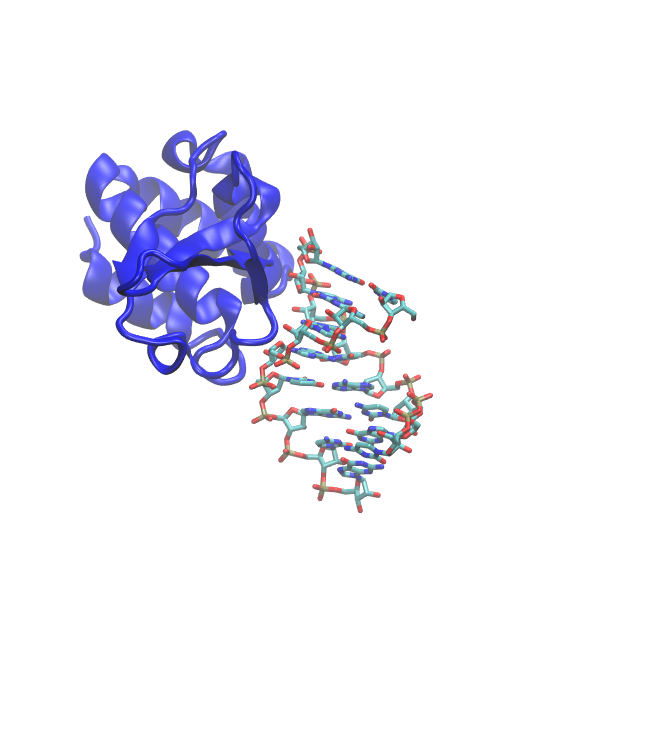
\includegraphics[width=0.9\linewidth,natwidth=610,natheight=642]{VP35_A.png}
%		\vspace{-40pt}
%		\caption{Chuỗi VP35 A bám vào \gls{dsrna} dài 8bps được tô màu xanh dương.}
%		\label{fig:vp35a}
%		\end{subfigure}
%		\\
%		\begin{subfigure}[h]{0.4\textheight}
%		\centering
%		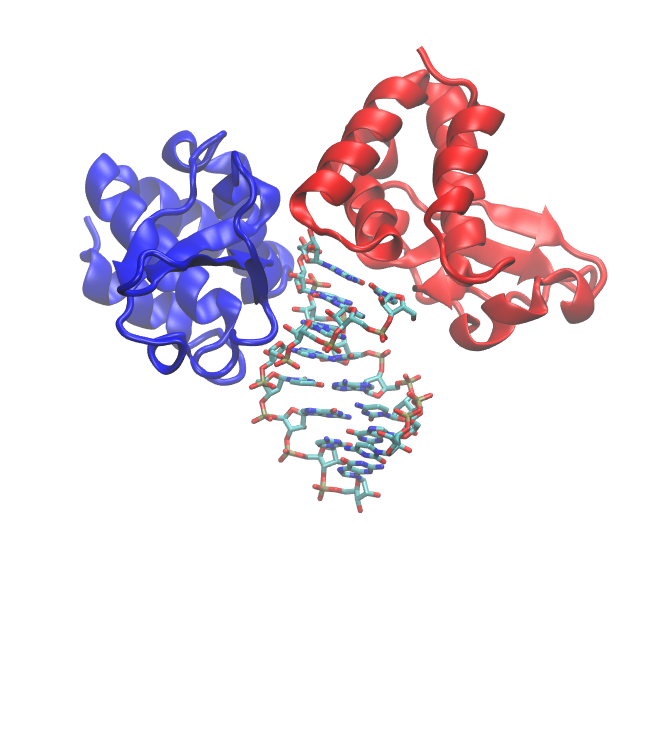
\includegraphics[width=1.0\linewidth,natwidth=610,natheight=642]{VP35_AB.png}
%		\vspace{-30pt}
%		\caption{2 chuỗi VP35 A và B bám vào \gls{dsrna} dài 8bps được tô màu xanh dương và đỏ.}
%		\label{fig:vp35ab}
%		\end{subfigure}
%		\clearpage
%
%		\caption{Cấu hình được khảo sát}
%		\end{figure}
		
	\subsection{B-conf}
	
		Gồm chuỗi B và dsRNA. B-conf giúp phân tích tương tác tại đầu chuỗi dsRNA của VP35. Đây là phân tử VP35 tương tác chính với \gls{dsrna} và có vai trò quan trọng trong tương tác giữa hệ các phân tử VP35 và \gls{dsrna}. Xem hình \ref{fig:vp35b}

%\newpage
\section{Phương pháp Mô phỏng động học phân tử}
Mô phỏng động lực học phân tử (Molecular Dynamics - MD) là một phương pháp hữu ích giúp tìm hiểu các tính chất vật lý của hệ phân tử sinh học.
	\subsection{Ý tưởng chính}
	
	Khi khảo sát một hệ nhiều hạt, người ta sử dụng các quy luật thống kê do không thể tìm được lời giải giải tích cho mọi tính chất của hệ. Với điều kiện hệ nhiều hạt này tuân theo giả thiết ergodic, việc khảo sát hệ theo thời gian có thể cho ta bức tranh sơ bộ về không gian phase của hệ.
	
	\Gls{md} cho biết quỹ đạo của từng nguyên tử trong hệ một cách cổ điển, tức là xem mỗi nguyên tử là mô hình một "hạt" tuân theo phương trình chuyển động Newton. Sau khi biết được quỹ đạo theo thời gian, các thông số như vận tốc, động năng, nhiệt độ,... sẽ được tính toán gián tiếp.
	
	%%%%%%%%%%%%%%%%%%%%%%%%%%%%% Bổ sung các bước MD %%%%%%%%%%%%%%%%%%%%%%%%%%%%%%%%%%%%%
	Cụ thể, các bước thuật toán dùng để mô phỏng động học phân tử gồm:
	\begin{enumerate}
	\item Đọc các tham số ban đầu: nhiệt độ, bước tính $\delta t$, nhóm cố định (restrained groups),...
	\item Chuẩn bị hệ: sử dụng tham số vận tốc, toạ độ đã có từ mô phỏng MD trước đó hoặc ngẫu nhiên chọn toạ độ và vận tốc đầu thoả phân bố Boltzmann.
	\item Tính toán lực tác dụng lên tất cả các nguyên tử, sử dụng trường lực (sẽ trình bày ở phần \ref{amberff}).
	\item Tích phân các phương trình chuyển động Newton. Thuật toán sử dụng thường là tích phân Verlet được trình bày ở phần \ref{verlet}. Trong bước này, các hiệu chỉnh cần thiết để kiểm soát nhiệt độ, áp suất, liên kết hoá học,... cũng được sử dụng. Khoá luận sẽ trình bày thuật toán kiểm soát nhiệt độ ở phần \ref{v-rescale}. Các phương trình chuyển động cần tính:
	\begin{align}
	m a_{i} = & \sum_{i}^{N} F_{i} \\
	%\label{force}
	v_{i} = & a_{i}\times dt \\
	\label{velocity}
	\vec{x}_{i} = & v_{i}\times dt
	%\label{coordinate}
	\end{align}
	\item Sau khi tính tích phân phương trình chuyển động, tính các đại lượng ta quan tâm như năng lượng, áp suất, nhiệt độ,... và ghi kết quả.
	\end{enumerate}
	
%	\subsection{Tham số sử dụng}
	\subsection{Trường lực}
	\label{amberff}
		\Gls{amber} là tên gọi của trường lực đặc trưng cho tương tác giữa các nguyên tử trong hệ. Tuy có tên gọi là "trường lực" nhưng nó không phải là đại lượng có thứ nguyên của lực. Trường lực (force field - ff) chính là hàm thế năng tương tác giữa các phân tử trong hóa học và sinh học tính toán. Sử dụng gần đúng cổ điển, người ta thường bỏ qua các ảnh hưởng gây ra bởi chuyển động của electron và xét năng lượng của hệ nguyên tử như hàm của các "hạt". Có rất nhiều ff được xây dựng. Các trường lực thường xuyên được sử dụng nhất được mang tên AMBER\cite{Duan2003,Cornell1995,Hornak2006,Ponder2003,Mackerell2004}, GROMOS\cite{Soares2005,Oostenbrink2004,Schmid2011,Schuler2001,Cornell1995}, CHARMM\cite{Mackerell2004,Cornell1995}, OPLS\cite{Mackerell2004,Cornell1995}. Với mỗi trường lực được phát triển còn có nhiều phiên bản khác nhau với mỗi ưu điểm riêng.
		
		Khóa luận đã sử dụng phiên bản \gls{amber} để mô phỏng tương tác giữa các phân tử vì đây là trường lực có rất nhiều ưu điểm trong việc mô tả hệ protein--RNA\cite{Hornak2006}. \Gls{amber} có đầy đủ tham số tương tác cho các nguyên tử trong phân tử RNA, protein, kể cả hydro không phân cực. Trong khi đó các trường lực united-atom xem các nguyên tử Hydro và Carbon trong mỗi methyl terminal và mỗi methylene bridge như một điểm tương tác duy nhất. Để mô phỏng thời gian dài, các trường lực thô (coarse-grained) được sử dụng.
		
		\Gls{amber} được mô tả bởi một hàm thế như sau:

		\begin{align}
		V(r^{N}) =& \sum_{ij}^{bond}k_{ij}\left(r_{ij} - r_{ij}^{0}\right)^{2} +\sum_{ijkl}^{dihedrals}k_{ijkl}\left[1+\cos\left(n_{ijkl}\phi_{ijkl}-\phi_{ijkl}^{0}\right)\right] +\nonumber\\
			&+ \sum_{ijkl}^{improper}\frac{1}{2} k_{\xi}\left[\xi_{ijkl}-\xi_{ijkl}^{0}\right]^{2} + \sum_{ijk}^{angles}k_{a}(\theta_{ijk}-\theta_{ijk}^{0})^{2}+ \sum_{ij}\left[\dfrac{q_{i} q_{j}}{\epsilon r_{ij}}+\dfrac{A_{ij}}{r_{ij}^{12}}-\dfrac{B_{ij}}{r_{ij}^{6}}\right]
		\label{ff}
		\end{align}
		\begin{figure}
		\begin{subfigure}{0.5\textwidth}
		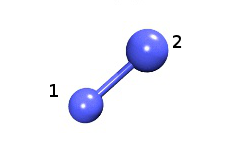
\includegraphics[width=0.7\textwidth,natwidth=610,natheight=642]{ff/12}
		\caption{Tương tác liên kết}
		\label{fig:12}
		\end{subfigure}
		\begin{subfigure}{0.5\textwidth}
		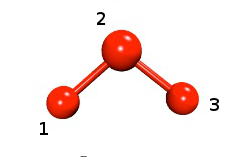
\includegraphics[width=0.7\textwidth,natwidth=610,natheight=642]{ff/13}
		\caption{Tương tác góc}
		\label{fig:13}
		\end{subfigure}\\
		\begin{subfigure}{0.5\textwidth}
		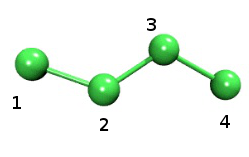
\includegraphics[width=0.7\textwidth,natwidth=610,natheight=642]{ff/14}
		\caption{Tương tác nhị diện}
		\label{fig:14}
		\end{subfigure}
		\begin{subfigure}{0.5\textwidth}
		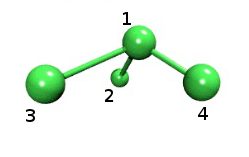
\includegraphics[width=0.7\textwidth,natwidth=610,natheight=642]{ff/impropers}
		\caption{Tương tác impropers}
		\label{fig:impropers}
		\end{subfigure}
		\caption{
		\label{fig:bond}%
		Tương tác giữa các nguyên tử có liên kết}
		\end{figure}
		Bốn tổng đầu (bốn tổng liên kết - bonded), lần lượt được lấy tổng theo:
		\begin{itemize}
		\item tất cả các liên kết trực tiếp (tương tác 1-2, xem hình \ref{fig:12})
		\item tất cả các góc (tương tác 1-3, xem hình \ref{fig:13})
		\item tất cả các góc nhị diện (tương tác 1-4, xem hình \ref{fig:14})
		\item tất cả các impropers (tương tác 1-4, xem hình \ref{fig:impropers})
		\end{itemize}
		Trong đó, tổng liên kết trực tiếp và các số hạng góc được biểu diễn như các dao động tử điều hòa đơn giản. Hai nguyên tử xem như dao động quanh một vị trí cân bằng.
		
		Các đại lượng $k_{ij}$,$r^{0}_{ij}$,$r_{ij}$ lần lượt là hệ số đàn hồi, độ dài liên kết ở vị trí cân bằng và độ dài liên kết thực tế giữa hai nguyên tử có liên kết hóa trị với nhau $i$ và $j$.
		
		Trong tổng theo các góc, $k_{ijk}$, $\theta^{0}_{ijk}$, $\theta_{ijk}$, lần lượt là hệ số đàn hồi, góc cân bằng và góc thực tế tạo bởi các nguyên tử $i $, $j $, $k $.
		
		Trong tổng theo góc nhị diện, $k_{ijkl}$, $\phi^{0}_{ijkl}$, $\phi_{ijkl}$ lần lượt là hằng số lực góc nhị diện, góc nhị diện cân bằng và góc nhị diện thực tế tạo bởi các nguyên tử $i$, $j$, $k$, $l$. Hệ số $n_{ijkl}$ là hằng số đối xưng nhận giá trị 1, 2 hoặc 3 ứng với số vị trí cực tiểu khi cho góc nhị diện quay một góc $360^{0}$.
		
		Tương tự, trong tổng theo các impropers, $k_{\xi}$, $\xi^{0}_{ijkl}$, $\xi_{ijkl}$ lần lượt là hằng số lực improper, góc improper cân bằng và góc improper thực tế tạo bởi các nguyên tử $i$, $j$, $k$, $l$.
		
		Các tổng cuối trong phương trình \eqref{ff} là các tổng không liên kết (non-bonded). Các tổng này bao gồm tương tác Van der Waals và tương tác tĩnh điện. Tương tác Van der Waals được mô tả bởi thế Lennard-Jones (6-12) và tương tác tĩnh điện được mô tả bởi thế Coulomb với giả thiết là điện tích điểm nằm tại tâm của nguyên tử \cite{Ponder2003}. Hằng số điện môi $\epsilon$ đặc trưng cho môi trường giữa hai nguyên tử, tham số $B_{ij}$ và $A_{ij}$ là các tham số 6-12 đặc trưng cho từng nguyên tố.
		
		Tất cả các hằng số lực, các tham số ứng với tọa độ cân bằng, các tham số 6-12 và hệ số đối xứng $n_{ijkl}$ được dẫn ra từ các tính toán lượng tử với độ chính xác cao và từ thực nghiệm\cite{Ponder2003}.

	\subsection{Thuật toán Verlet sử dụng trong mô phỏng MD}
	\label{verlet}
		Trong quá trình giải phương trình chuyển động Newton bằng phương pháp số, có một thủ thuật nhằm tính đại lượng tọa độ của hệ hạt với bậc chặt cụt cao hơn so với những phương pháp thông thường.
		
		Tích phân Verlet\cite{Verlet1967} là một phương pháp tính toán số được sử dụng trong phương trình chuyển động Newton. Nó thường dùng để tính quỹ đạo của hạt trong mô phỏng động học và đồ họa máy tính. Thuật toán được phát triển bởi Delambre (1791) và được Verlet sử dụng nhiều trong động học phân tử những năm 60. Nó cũng được dùng để tính toán quỹ đạo sao chổi Halley.
			
		Tích phân Verlet có tính hội tụ cao, có tính chất suy ngược (time-reversible), tính bảo toàn của hệ ngẫu đối của không gian pha và không tốn quá nhiều bước tính so với thuật toán Euler.
			
		Thay vì tính trực tiếp phương trình \eqref{velocity} để tìm toạ độ $\vec{x}_i$, sử dụng khai triển Taylor đến bậc 3 của tọa độ hạt theo thời gian ta được hai phương trình sau:
		\begin{align}
		\vec{x}\left(t+\Delta t\right) &=\vec{x}\left(t\right)+\vec{v}\left(t\right)\Delta t + \dfrac{\vec{a}\left(t\right)\Delta t^{2}}{2} + \dfrac{\vec{b}\left(t\right)\Delta t^{3}}{6} + \mathcal{O}\left(\Delta t^{4}\right)\\
		\vec{x}\left(t-\Delta t\right) &=\vec{x}\left(t\right)-\vec{v}\left(t\right)\Delta t + \dfrac{\vec{a}\left(t\right)\Delta t^{2}}{2} - \dfrac{\vec{b}\left(t\right)\Delta t^{3}}{6} + \mathcal{O}\left(\Delta t^{4}\right)
		\label{verlet1}
		\end{align}
		Cộng hai vế hai phương trình trên, rút ra được:
		\begin{equation}
		\vec{x}\left(t+\Delta t\right)=2\vec{x}\left(t\right)-\vec{x}\left(t-\Delta t\right)+\vec{a}\left(t\right)\Delta t^{2}+\mathcal{O}\left(\Delta t^{4}\right)
		\label{verlet2}
		\end{equation}
		Từ phương trình \eqref{verlet2}, có thể thấy rằng tích phân Verlet đem lại bậc sai số cao hơn nhiều so với phương pháp Euler.
	\subsection{Thuật toán kiểm soát nhiệt độ}
	\label{v-rescale}
		Để có thể mô phỏng (i) hệ phân tử lớn trong (ii) thời gian dài sao cho kết quả mô phỏng phù hợp với thực nghiệm, người ta tìm các thuật toán để có thể kiểm soát các đại lượng nhiệt động như mong muốn. Cụ thể, người ta áp dụng mô hình Vi chính tắc, cùng các điều kiện ràng buộc tương ứng để mô phỏng hệ (số hạt, thể tích, năng lượng tổng của hệ không đổi theo thời gian). Nhưng mô hình Vi chính tắc này vẫn chưa đem lại những quan sát có được trong thực nghiệm, người ta sử dụng mô hình Chính tắc để mô tả hệ với mong muốn nhận được những kết quả phù hợp với thực nghiệm hơn. Thuật toán đơn giản có thể kiểm soát nhiệt độ của hệ thông qua kiểm soát vận tốc của hạt trong hệ được gọi chung là V-rescale.
		
		Có nhiều phương pháp khác nhau để kiểm soát nhiệt độ của hệ. Khóa luận chỉ sử dụng phương pháp Berendsen và Nosé-Hoover nên sẽ chỉ trình bày sơ lược hai phương pháp này\cite{Bussi2007}.
		
		Một cách tổng quát, kiểm soát nhiệt độ thông qua kiểm soát vận tốc hạt trong hệ dựa trên mối liên hệ giữa nhiệt độ và vận tốc hạt được trình bày trong phương trình \eqref{vT} sau:
		\begin{equation}
		\sum_{i=1}^{N} \dfrac{\vec{p}_{i}}{2m_{i}} = \dfrac{k_{b}T}{2}\left(3N-N_{c}\right)
		\label{vT}
		\end{equation}
		với $3N - N_{c} = N_{df}$ là số bậc tự do.
		Để thực hiện được việc điều chỉnh nhiệt độ về một giá trị cho trước thông qua điều chỉnh $\Delta T$, ta sử dụng tham số $\lambda$ như sau:
		\begin{align}
		\Delta T = & \dfrac{1}{2} \sum 2\dfrac{m_{i}\left(\lambda v_{i}\right)^{2}}{N_{df} k_{B}} - 2\dfrac{m_{i} v_{i}^{2}}{N_{df} k_{B}}\\
		\Delta T = & \left(\lambda^{2} - 1\right) T\left(t\right)\\
		\lambda = &  \sqrt{\dfrac{T_{0}}{T\left(t\right)}}
		\end{align}
		Chỉ việc nhân vận tốc hạt trong mỗi bước lặp với $\lambda$ vừa tính được ở bước liền trước thì vận tốc của các hạt sẽ dần dần phân bố một cách tương ứng với nhiệt độ $T_{0}$.
		
		Việc kiểm soát nhiệt độ một cách chặt chẽ bởi tham số $\lambda$ khiến cho thăng giáng nhiệt bị bóp hẹp và cần thiết sử dụng các phương pháp hiệu chỉnh ở cấp độ cao hơn.
		\subsubsection{Phương pháp Berendsen}
		
			Ta có thể hình dung sơ lược về phương pháp này như sau:
			\begin{itemize}
			\item Phương pháp Berendsen chủ yếu được dùng để đưa hệ về một nhiệt độ ổn định, nhưng hệ không có tính chất thăng giáng nhiệt của hệ Chính tắc.
			\item Sau mỗi bước lặp, vận tốc của hạt trong hệ thay đổi và làm thay đổi nhiệt độ của hệ một lượng $\Delta T$. Thuật toán sẽ giúp điều chỉnh độ thay đổi này sao cho nhiệt độ ổn định quanh giá trị $T_{0}$.
			\item Băng cách hiệu chỉnh như trên, có thể thực hiện quá trình mô phỏng trong thời gian dài mà vẫn tránh được dịch chuyển mức năng lượng sinh ra bởi sai số của phép tính toán số.
			\item Hệ mô phỏng có thể được chọn một cách tối giản để giảm thiểu tài nguyên tính toán, do sai số đã được giảm thiểu.
			\end{itemize}
			Thay vì tính tham số $\lambda$ một cách trực tiếp như trước, người ta tìm cách để nhiệt độ $T$ có thể thăng giáng quanh một giá trị với biên độ thăng giáng có thể đánh giá được qua tham số $\tau$ như sau:
			\begin{equation}
			\dfrac{dT\left(t\right)}{dt} = \dfrac{1}{\tau}\left(T_{0}-T\left(t\right)\right)
			\label{exp-v-r}
			\end{equation}
			Ở đây, $\tau$ được gọi là tham số cặp nhiệt độ (T-coupling). Gọi như vậy vì nó cho thấy tương tác giữa hệ và bể nhiệt trao đổi nhiệt với nhau nhanh hay không. Với cách kiểm soát nhiệt độ như vậy, nhiệt độ của hệ hội tụ theo hàm số mũ và thu được hệ số $\lambda$ cho vận tốc hạt như sau:
			\begin{equation}
			\lambda^{2} = 1 + \dfrac{\delta t}{\tau}\left[\dfrac{T_{0}}{T\left(t-\delta t\right)}-1\right]
			\end{equation}
			Hiệu chỉnh $\tau$ một cách kỹ lưỡng sẽ cho phép nhiệt độ $T$ tiến đến giá trị $T_{0}$ cho trước với thăng giáng nhiệt thu được từ phương trình sau:
			\begin{equation}
			\Delta T = \dfrac{\delta t}{\tau}\left(T_{0}-T\left(t\right)\right)
			\end{equation}
			Với $t\rightarrow \infty$ thì hệ hạt có các tính chất của hệ Vi chính tắc, không có hiệu chỉnh Berensend tham gia vào quá trình mô phỏng. Nhưng với giá trị $\tau \sim \delta t$ thì hệ số $\lambda$ trở về với giá trị như đã trình bày ở phần tổng quát của V-rescale.
			
			Trong chương trình mô phỏng mà đề tài sử dụng, $\tau$ được hiệu chỉnh về giá trị $0.4\delta t$.
			
			Từ phương trình \eqref{exp-v-r} có thể thấy rằng nhiệt độ $T$ của hệ tiến về giá trị $T_{0}$ theo hàm mũ. Như vậy, hệ sẽ tiến về mô hình Vi chính tắc, thay vì tiến về mô hình Chính tắc mà ta mong muốn.
		\subsubsection{Phương pháp Nosé-Hoover}
		
			Để khắc phục các nhược điểm của phương pháp Berendsen, Nosé phát triển một phương pháp khác nhằm mở rộng hệ bằng cách xem bể nhiệt như một phần bổ sung của hệ hạt đang xét, nhờ thêm vào biến phụ $\bar{s}$, cũng như giả khối lượng $Q$ ($>>0$) và giả vận tốc $\dot{\bar{s}}$. Cụ thể, biến thời gian được hiệu chỉnh lại như sau:
			\begin{equation}
			d\bar{t}=\bar{s} dt
			\end{equation}
			Các biến tọa độ không gian của hệ hạt vẫn không bị thay đổi, theo đó:
			\begin{align}
			\bar{\vec{r}} = & \vec{r}\\
			\bar{\dot{\vec{r}}} = & \bar{s}^{-1}\dot{\vec{r}}\\
			\bar{s} = & s^{-1}\\
			\dot{\bar{s}} = & \bar{s}^{-1}\dot{\bar{s}}
			\end{align}
			Sử dụng bốn hệ thức biến đổi tọa độ trên, ta có thể xây dựng được Lagrangian:
			\begin{equation}
			\mathcal{L}=\sum_{i} \dfrac{m_{i}}{2}\bar{s}^{2}\dot{\bar{\vec{r}}}_{i} - U\left(\bar{r}\right) + \dfrac{1}{2}Q\dot{\bar{s}}^{2} - gk_{B}T_{0}\ln \bar{s}
			\label{lagrangian}
			\end{equation}
			với $g=N_{df}$.
			Quan sát phương trình \eqref{lagrangian} dễ dàng thấy được số hạng động năng bây giờ gồm tổng động năng có được do chuyển động của hạt và động năng sinh bởi biến phụ $\dot{\bar{s}}$ và thế năng gồm thế năng thực của hệ hạt cộng với thế năng phát sinh bởi biến phụ $\bar{s}$. Theo đó, năng lượng thực của hệ hạt mà ta đang quan sát (gồm động năng và thế năng của hệ hạt) không còn là hằng số mà thay đổi theo $\bar{s}$. Điều đó có nghĩa là sử dụng Lagrangian vừa xây dựng được, ta có thể mô tả hệ hạt trao đổi nhiệt với bể nhiệt.
			
			Phương trình chuyển động có dạng:
			\begin{eqnarray}
			\label{r_bar}
			\ddot{\bar{\vec{r}}}_{i} = & \dfrac{\bar{\vec{F}}_{i}}{m_{i}\bar{s}^{2}} - \dfrac{2\dot{\bar{s}}\dot{\bar{\vec{r}}}_{i}}{\bar{s}}\\
			\ddot{\bar{s}} = & \dfrac{1}{Q\bar{s}}\left( \sum_{i}m_{i}\bar{s}^{2}\dot{\bar{\vec{r}}}_{i} - gk_{B}T_{0} \right)
			\label{s_bar}
			\end{eqnarray}
			Đây là phương trình chuyển động của hệ hạt trong hệ tọa độ suy rộng $\left( \bar{r},\bar{p},\bar{t} \right)$. Tuy nhiên, \eqref{s_bar} là phương trình đạo hàm bậc 2 theo thời gian và $\bar{s}$ có xu hướng dao động tuần hoàn, nên thăng giáng nhiệt cũng mang tính chu kỳ.
			
			Nosé và Hoover đã tìm cách biến đổi lại phương trình \eqref{r_bar} trở về phương trình sử dụng hệ tọa độ thực, và phương trình \eqref{s_bar} trở về phương trình đạo hàm bậc nhất theo thời gian, sử dụng các hệ thức biến đổi sau:
			\begin{align}
			s = \bar{s},\quad \dot{s} = \bar{s}\dot{\bar{s}},\quad \ddot{s} = \bar{s}^2\ddot{\bar{s}}+\bar{s}\dot{\bar{s}}^2,\\
			\vec{r} = \bar{\vec{r}},\quad \dot{\vec{r}}=\bar{s}\dot{\vec{r}},\quad \ddot{r} = \bar{s}^{2}\ddot{\bar{\vec{r}}} + \bar{s}\dot{\bar{\vec{r}}}^{2}
			\end{align}
			và thay
			\begin{equation}
			\gamma = \dfrac{\dot{s}}{s}
			\end{equation}
			phương trình chuyển động \eqref{s_bar} được viết lại thành:
			\begin{align}
			\ddot{\vec{r}}_{i}= & \dfrac{\vec{F}_{i}}{m_{i}} - \gamma \vec{r}_{i},\\
			\dot{\gamma}= & \dfrac{-k_{B}N_{df}}{Q}T\left(t\right) \left( \dfrac{T_{0}}{T\left(t\right)}-1 \right)
			\label{gamma}
			\end{align}
			Đặt $\tau_{relax} = \dfrac{Q}{N_{df}k_{B}T_{0}}$ là thời gian phục hồi đặc trưng cho chu kỳ dao động nhỏ của biến $\bar{s}$ thì phương trình \eqref{gamma} có thể viết lại:
			\begin{equation}
			\dot{\gamma} = -\dfrac{1}{\tau_{relax}}\left( \dfrac{T_{0}}{T\left(t\right)}-1 \right)
			\end{equation}
			Trong phương trình \eqref{gamma}, khối lượng ảo $Q$ cần được chọn một cách phù hợp. Hệ trở thành hệ Vi chính tắc nếu cho $Q\rightarrow \infty$. Nếu chọn Q quá lớn, sẽ phải mô phỏng trong thời gian dài mới đạt được phân bố Chính tắc. Ngược lại, chọn $Q$ quá nhỏ sẽ dẫn đến tần số nhiễu loạn của hệ hạt trong không gian thực là rất lớn, và ta không quan sát được sự trao đổi động năng giữa bể nhiệt và hệ phân tử đang quan sát.
			
			Trong thực tế, hệ phân tử mô phỏng thường có khối lượng khác nhau tùy theo nguyên tố. Để chọn được $Q$, cần thiết phải chọn giá trị $Q$ với mỗi nhóm phân tử khác nhau để thời gian mô phỏng là tối thiểu mà hệ vẫn đạt được phân bố chính tắc. Cách chọn Q theo nhóm được trình bày cụ thể hơn trong phần \ref{rcutoff}
%	\subsection{}
\section{\glsentryfull{smd}}
Chính là \gls{md} nhưng đặt thế năng phụ thuộc vào thời gian lên các nhóm phân tử xác định để tách các nhóm này ra. Việc tách hai nhóm phân tử ra có tác dụng hỗ trợ kiểm tra giả thiết về chuyển trạng thái của hệ phân tử. Một cách cụ thể, \gls{smd} áp dụng đối với \gls{ligand} và \gls{receptor} sẽ giúp quan sát quá trình hai nhóm phân tử này tách ra khỏi nhau. Đây là một quá trình xảy ra trong thực tế, tuy nhiên cần khảo sát hệ trong thời gian rất dài mới có thể ngẫu nhiên quan sát được quá trình này. Do đó, \gls{smd} được sử dụng với mục đích giảm thiểu thời gian mô phỏng mà vẫn giúp quan sát hệ chuyển trạng thái ra sao.

Có hai cách xác định tham số của thế năng, tương ứng với hai cách "kéo" các nhóm phân tử ra: kéo với lực kéo không đổi hoặc kéo nhóm tách ra với vận tốc không đổi. Đề tài sử dụng phương pháp kéo với vận tốc không đổi\cite{Lu1998}. Trong suốt quá trình kéo, dễ dàng để tính toán lực kéo các nhóm. Từ đó phác thảo được tương tác giữa các nhóm phân tử. Hơn nữa, có thể xác định được độ thay đổi năng lượng khi hệ phân tử chuyển từ trạng thái trước khi kéo sang trạng thái sau khi kéo.

%%%%%%%%%%%%%%%%%%%%%%%%%%%%%%%%%%%%%%%% Bổ sung hình rupture force và các hình SMD từ bài báo của thầy Lý %%%%%%%%%%%%%%%%%%%%

	\subsection{\glsentrytext{smd} sử dụng lực kéo không đổi}
	
	Bằng cách cộng thêm lực kéo với độ lớn không đổi vào nhóm các phân tử cần kéo và thực hiện quá trình mô phỏng. Đối với nhóm phân tử không cần kéo, cần cố định một cách tương đối vị trí của chúng, nhằm tránh việc bị kéo theo do tương tác với nhóm phân tử được kéo ra. Thực hiện \gls{smd} nhiều lần với giá trị lực kéo khác nhau giúp xác định lực tương tác giữa hai nhóm phân tử nằm trong khoảng giá trị nào. Qua đó, có thể đánh giá sơ bộ tương tác giữa hai nhóm phân tử (ví dụ \gls{ligand} và \gls{receptor} được nêu ở trên).
	\begin{wrapfigure}{r}{0.4\textwidth}
	\vspace{-30pt}
	\begin{center}
	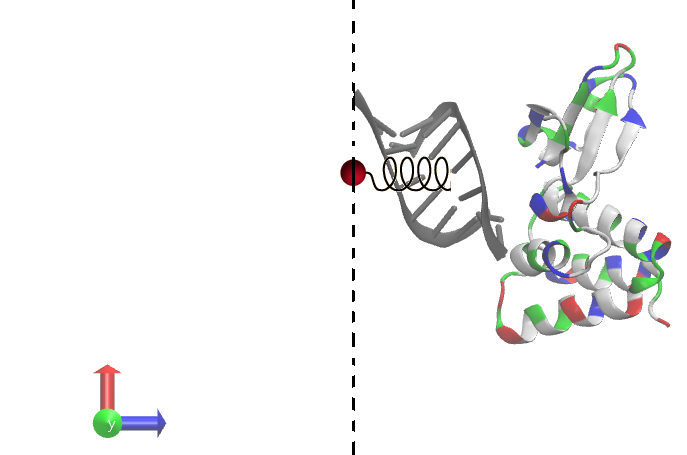
\includegraphics[width=0.4\textwidth,natwidth=610,natheight=642]{smd-1}\\
	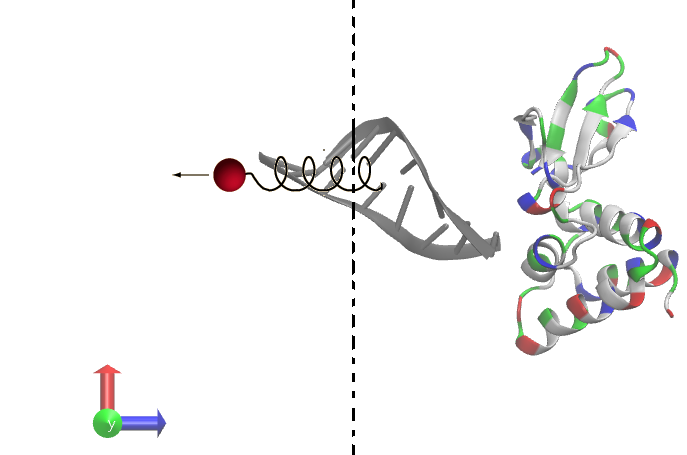
\includegraphics[width=0.4\textwidth,natwidth=610,natheight=642]{smd-2}\\
	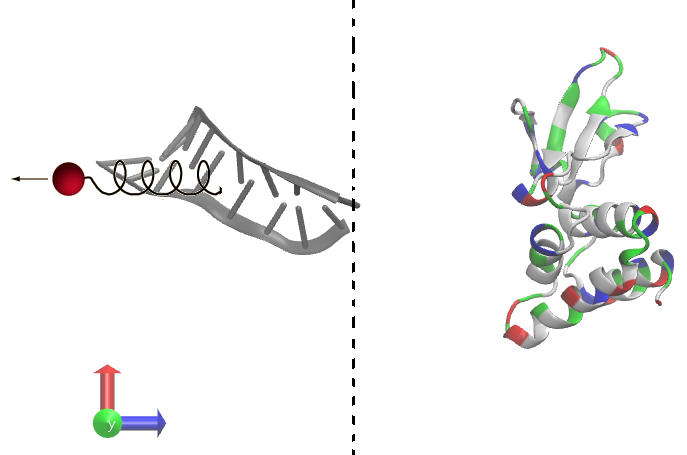
\includegraphics[width=0.4\textwidth,natwidth=610,natheight=642]{smd-3}
	\end{center}
	\vspace{-5pt}
	\caption{Bằng cách di chuyển nhóm liên kết (constraint group) với vận tốc không đổi, lực tác động lên nhóm phân tử cần kéo ra sẽ lớn dần đến một giá trị đủ để tách nhóm đó ra.}
	\label{fig:smd}
	\end{wrapfigure}
	\subsection{\glsentrytext{smd} sử dụng vận tốc kéo không đổi}
	Có thể hình dung về cách kéo nhóm phân tử như hình \ref{fig:smd} được trình bày dưới đây:
	Thế năng đàn hồi đặt lên nhóm phân tử cần kéo có dạng như sau:
	\begin{equation}
	U\left(\vec{r}\right) = \dfrac{1}{2} k\left[ vt - \left( \vec{r}-\vec{r}_{0} \right) \dot\vec{n} \right]^{2}
	\end{equation}
	với $k$ là hệ số đàn hồi, $v=constant$ là tốc độ di chuyển của nhóm liên kết, $\vec{r}$ là vị trí của hạt được kéo và $\vec{r}_{0}$ là vị trí ban đầu của hạt, $\vec{n}$ là hướng kéo.
	
	Cách kéo nhóm phân tử này có ưu điểm so với áp dụng lực kéo không đổi là không phải thực hiện rà soát quá nhiều giá trị lực kéo để ước lượng lực tương tác giữa hai nhóm phân tử. Hơn nữa, công trung bình tác dụng lên hệ sẽ tiến đến một giá trị xác định, do nhóm liên kết di chuyển với vận tốc không đổi và công tác dụng lên hệ (một cách tương đối) sẽ bằng năng lượng liên kết giữa hai nhóm và thế năng đàn hồi $U\left( \vec{r}\right) $ trung bình và động năng trung bình của nhóm phân tử kéo. Nói cách khác, hệ sẽ ít bị can thiệp một cách "thô bạo" hơn so với cách kéo sử dụng lực không đổi được trình bày ở trên.
\section{Tham số sử dụng trong các quá trình mô phỏng}
Mô phỏng đã được thực hiện 3 lần đối với mỗi phân tử 3L25 (VP35 tự nhiên), 3L27 (đột biến \gls{R312A}), 3L28 (đột biến \gls{K339A}) và phân tử VP35 đột biến \gls{K282A}.

Hệ gồm 200000 nguyên tử. Mô hình phân tử nước được sử dụng là TIP-4P \cite{Horn2004}. Hệ phân tử được phân làm hai nhóm khi đưa nhiệt độ vào hệ thông qua khối lượng ảo Q tương ứng: Protein và không phải Protein (Protein group \& non-Protein group).
Các bước chạy mô phỏng được thực hiện:
\begin{enumerate}
\item Cực tiểu hóa năng lượng hệ phân tử
\item Mô phỏng trạng thái (NVT) của hệ không đổi
\item Mô phỏng trạng thái (NPT) của hệ không đổi
\item Mô phỏng \gls{smd}. Các bước trước đó được xem như các bước thiết lập hệ mô phỏng thể thực hiện mô phỏng \gls{smd}
\end{enumerate}
\subsubsection{Cực tiểu hóa năng lượng}
Nhằm mục đích để hệ hạt có vị trí ổn định nhất và không có những "va đập" quá mạnh. Cụ thể, hệ phân tử phân bố trong không gian sao cho thế năng tổng của hệ là thấp nhất. Điều kiện dừng chương trình: lực tối đa tác dụng lên hạt bằng $1000\ kJ/mol/nm$. Cách tính tương tác Coulomb ở khoảng cách xa: Particle Mesh Ewald (PME). Bán kính chặt cụt đối với tương tác Coulomb và Van der Waals là $r_{Coulomb}=1nm$ và $r_{VdW}=1nm$.
\label{rcutoff}
\subsubsection{Cân bằng chính tắc (NVT)}
Các thông số bán kính chặt cụt và phương pháp tính tương tác Coulomb ở khoảng cách xa vẫn như trên. Áp dụng phương pháp Berendsen để ổn định nhiệt độ của hệ tại $300K$ với $\tau_{t}=0.1\left(ps\right)$. Vận tốc của hạt được đưa vào và ổn định một cách ngẫu nhiên sao cho thoả phân bố Maxwell. Áp dụng thuật toán Verlet để giải phương trình chuyển động. Thời gian mô phỏng bước cân bằng NVT là $100\left(ps\right)$.
\subsubsection{Cân bằng đẳng nhiệt - đẳng tích (NPT)}
Các thông số vẫn tương tự như trên. Để ổn định áp suất của hệ tại $1 \left(bar\right)$, sử dụng phương pháp Parrinello-Rahman với $\tau_{p}=2\left(ps\right)$, hằng số nén $\beta=-\frac{1}{V}\frac{\partial V}{\partial p} = 4.5\times 10^{-5}\left(bar^{-1}\right)$. Thời gian mô phỏng bước cân bằng NPT là $100\left(ps\right)$.
\subsubsection{\glsentrytext{smd}}
Bán kính chặt cụt được sử dụng trong bước này là $1.4\left(nm\right)$. Tốc độ di chuyển của nhóm liên kết (constraint group) bằng $5\left(nm/ns\right)$. Lực sử dụng để kéo là $1000\ \left( kJ . mol^ {-1} nm^ {-2} \right)$.
\section{Các công cụ phân tích kết quả}
	\subsection{Lực kéo tối đa}
	%%%%%%%%%% Insert Rupture force figure here %%%%%%%%%%%%%%%%%%%%%%%
	\begin{figure}[t!]
	\centering
	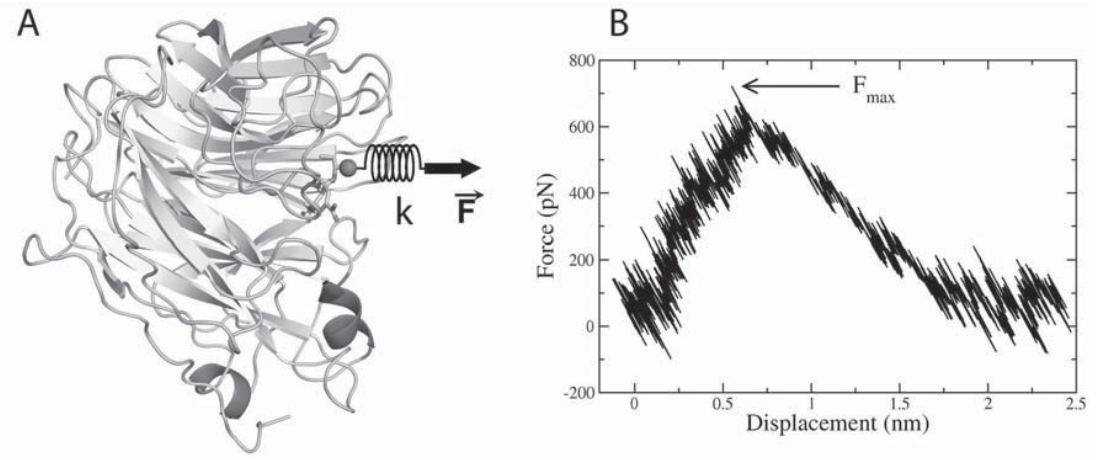
\includegraphics[width=0.7\textwidth,natwidth=610,natheight=642]{pull-force}
	\caption{\textbf{(A)} kéo ligand ra khỏi protein bằng cách đặt một thế năng điều hoà thay đổi theo thời gian, tương đương với việc đặt một lực kéo của một lò xo với hệ số đàn hồi \textit{k} lên ligand. \textbf{(B)} Đường biểu diễn lực kéo theo toạ độ. Lực kéo tối đa $F_{max}$ đặc trưng cho ái lực liên kết giữa ligand và protein. Nguồn \cite{SuanLi2012}}
	\label{fig:rupture-force}
	\end{figure}
	Là lực lớn nhất dùng để kéo hai phân tử ra trong suốt quá trình mô phỏng. Do hệ phân tử đã ở vị trí ứng với đáy của giếng thế địa phương, nên để tách hai nhóm phân tử protein và \gls{dsrna} ra thì lực dùng để tách hai nhóm ra sẽ lớn dần đến một giá trị mà tại đó hai nhóm không còn tương tác đáng kể với nhau nữa.
	Việc so sánh lực kéo tối đa giữa các nhóm phân tử giúp đánh giá tương đối tương tác giữa các nhóm phân tử này. Điều này đặc biệt có ý nghĩa khi so sánh lực kéo các cấu hình đột biến một \gls{residue} để tìm hiểu vai trò của nó trong tương tác giữa các nhóm.
	%%%%%%%%%%%%%%%%%%%%%%%%%%%%%%%%%%%%%%%%%%%%%%%%%%%% Bổ sung hình Rupture force ở đây %%%%%%%%%%%%%%%%%%%%%%%%%%
	\begin{figure}[h!]
	\centering
	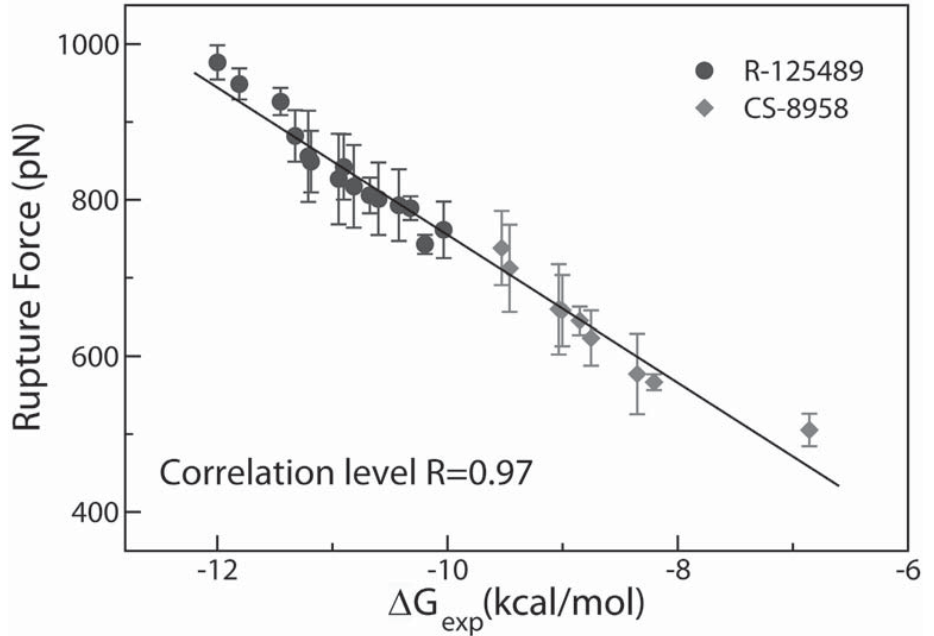
\includegraphics[width=0.7\textwidth,natwidth=610,natheight=642]{rupture_force-delta_G}
	\caption{Đồ thị tương quan giữa lực kéo tối đa (Rupture Force) và năng lượng tương tác giữa phân tử R-125489 với thụ thể NA của virus cúm và giữa phân tử CS-8959 với thụ thể NA của virus cúm \cite{SuanLi2012}. Hệ số tương quan (correlation level) R = 0.97}
	\label{fig:rupture-force-delta-g}
	\end{figure}
	\subsection{Thế năng tương tác theo thời gian}
	
	Từ các tham số toạ độ và từ \gls{amber} đã được định nghĩa, có thể dễ dàng tính lại được đóng góp của tương tác Coulomb hoặc tương tác Van der Waals vào tương tác của một \gls{residue}. Điều này giúp đánh giá một cách tương đối vai trò của các \gls{residue}, đồng thời giúp dự đoán các amino acid có khả năng đóng góp cho tương tác giữa \gls{dsrna} và VP35.
	%%%%%%%%%%%%%%%%%%%%%%%%%% Bổ sung biểu thức tính thế năng ở đây %%%%%%%%%%%%%%%%%%%%%%%%%%%%%%%%%%%%%%%%%%%%%%%%
	Một cách cụ thể, thành phần tương tác Coulomb có dạng:
	\begin{equation}
	V_{i}\left(t\right) = \sum_{j}\left[\dfrac{q_{i} q_{j}}{\epsilon r_{ij}}\right]
	\end{equation}
	và thành phần tương tác theo thế Lennard-Jones có dạng:
	\begin{equation}
	V_{i}\left(t\right) = \sum_{j}\left[\dfrac{A_{ij}}{r_{ij}^{12}}-\dfrac{B_{ij}}{r_{ij}^{6}}\right]
	\end{equation}
	\subsection{Liên kết Hydro}
	%%%%%%%%%%%%%%%%%%%%%%%%%%%%%%%%%%%%%%% Warning!!!! check GROMACS manual!!!!! %%%%%%%%%%%%%%%%%%%%%%%%%%%%%%%%%%%
	\begin{figure}[h]
	\centering
	\includegraphics[width=0.3\textwidth,natwidth=610,natheight=642]{hbond}
	\caption{Khoảng cách và góc giữa phân tử Donor, Acceptor và nguyên tử Hydro}
	\label{fig:hbond_angle}
	\end{figure}
	Liên kết Hydro (H-bond) là liên kết đóng góp rất nhiều cho tương tác giữa hai nguyên tử. Đặc biệt trong môi trường nước, liên kết Hydro là liên kết chiếm ưu thế.
	Liên kết Hydro là liên kết giữa nguyên tử phân cực dương (donor) và nguyên tử phân cực âm (acceptor) thỏa điều kiện (i) cách nhau một khoảng 3.5\AA{} và (ii) góc nhị diện tạo bởi donor và acceptor là lớn hơn hoặc bằng $ 30^{0} $. Xem hình \ref{fig:hbond_angle}.
%%%%%%%%%%%%%%%%%%%%%%%%%%%%%%%%%%%%%%%%%%%
%+ Ket thuc Chuong 2.
%%%%%%%%%%%%%%%%%%%%%%%%%%%%%%%%%%%%%%%%%%%


\newpage
\pagestyle{fancy}
%%%%%%%%%%%%%%%%%%%     Chuong 3       %%%%%%%%%%%%%%%%%%%%%%%%
%%%%%%%%%%%%%%%%%%%                    %%%%%%%%%%%%%%%%%%%%%%%%
\setcounter{chapter}{2}
\chapter{Kết quả và thảo luận}
%\section{A-conf}

%%%%%%%%%%%%%%%%%%%%%%%%%%%%%%%%%%%%%%%%% Bổ sung kết quả setup hệ: Minimize Eenergy (E), NVT (Temp), có thể NPT. Đồ thị distance khi kéo, biện luận %%%%%%%%%%%%%%%%%%%%%%%%%%%
\section{Thiết lập hệ mô phỏng}
	\subsection{Cực tiểu hoá năng lượng}
	\begin{figure}[h]
	\centering
	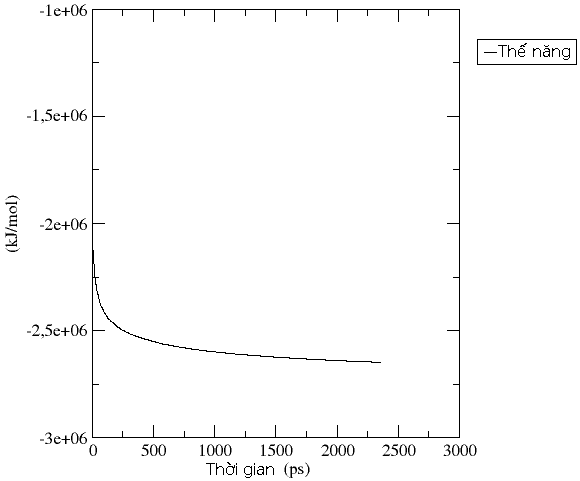
\includegraphics[width=0.7\textwidth,natwidth=610,natheight=642]{25energy}
	\caption{Đồ thị thế năng của hệ theo thời gian trong bước cực tiểu hoá năng lượng.}
	\label{fig:em}
	\end{figure}
	Như đã trình bày trong chương trước, đây là bước chạy mô phỏng giúp hệ hạt phân bố một cách ổn định trong không gian. Quan sát đồ thị \ref{fig:em} có thể thấy thế năng của hệ giảm theo thời gian. Điều này có nghĩa các nguyên tử trong hệ dần dần "chuyển" về các vị trí sao cho tương tác lực lên lẫn nhau là tối thiểu. Cụ thể, thế năng của hệ sau quá trình cực tiểu hoá năng lượng là dưới $-2.5\times 10^{-6} kJ/mol$. Đây là một con số thường thấy đối với các hệ mô phỏng. Điều kiện để dừng phép mô phỏng chính là \emph{lực lớn nhất tác dụng lên bất kỳ nguyên tử nào trong hệ phải nhỏ hơn $1000\  kJ.mol^{-1}.nm^{-1}$ }. Đây là điều kiện cần, bảo đảm các nguyên tử tương tác với nhau với giá trị lực không quá lớn. Xem xét các dữ liệu xuất ra từ quá trình mô phỏng (cụ thể, dữ liệu từ file \textbf{em.log}) thu được lực có giá trị lớn nhất là lực đặt lên nguyên tử thứ 210: $999 kJ.mol^{-1}.nm^{-1}$.
	\subsection{Cân bằng chính tắc (NVT)}
	\begin{figure}[h]
	\centering
	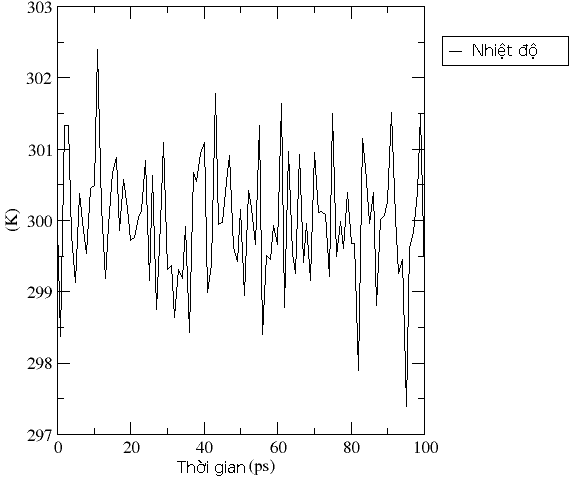
\includegraphics[width=0.7\textwidth,natwidth=610,natheight=642]{25temperature}
	\caption{Nhiệt độ trung bình của hệ theo thời gian trong bước cân bằng chính tắc (NVT)}
	\label{fig:nvt}
	\end{figure}
	Ở bước này, các nguyên tử ở chuỗi chính ($C_{\alpha}$--$C_{\beta}$) được giữ cố định và nhiệt độ được đưa dần vào hệ thông qua điều khiển động năng của hệ như đã trình bày ở phần \ref{v-rescale}. Từ đồ thị rút ra được thăng giáng nhiệt trung bình của hệ khoảng $1\%$.
	\subsection{Cân bằng đẳng nhiệt - đẳng tích (NPT)}
	\begin{figure}[h]
	\centering
	\begin{subfigure}{0.45\textheight}
	\centering
	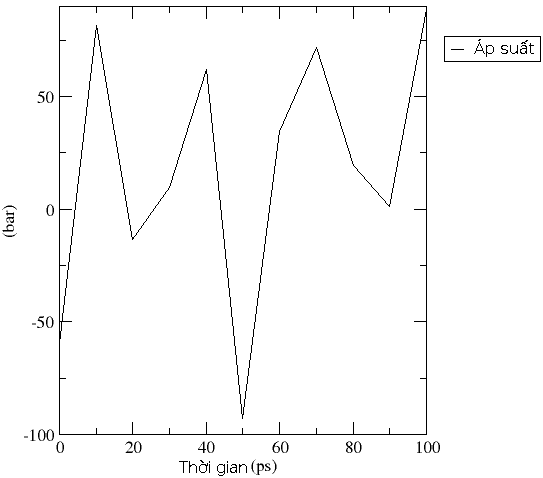
\includegraphics[width=0.7\textwidth,natwidth=610,natheight=642]{25pressure2}
	\caption{Áp suất của hệ theo thời gian trong bước cân bằng đẳng nhiệt - đẳng tích (NPT)}
	\label{fig:pressure}
	\end{subfigure}
	\begin{subfigure}{0.45\textheight}
	\centering
	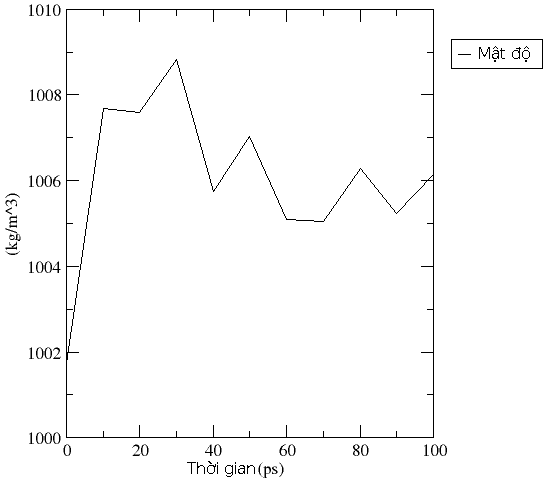
\includegraphics[width=0.7\textwidth,natwidth=610,natheight=642]{25density2}
	\caption{Mật độ của hệ theo thời gian trong bước cân bằng đẳng nhiệt - đẳng tích (NPT)}
	\label{fig:density}
	\end{subfigure}
	\end{figure}
	Đồ thị \ref{fig:pressure} cho thấy áp suất của hệ mô phỏng thay đổi theo thời gian với biên độ lớn, nhưng nếu lấy trung bình áp suất theo thời gian dài thì giá trị trung bình này lại không lớn. Đồ thị \ref{fig:density} cho thấy mật độ khối lượng của hệ vào khoảng $1006 kg/m^{3}$. Giá trị này tương đối phù hợp với mô hình nước TIP-4P\cite{Horn2004} đã được sử dụng.
\section{Khoảng cách giữa \glsentrytext{dsrna} và VP35 theo thời gian}
\label{distance}
\begin{figure}[h]
\centering
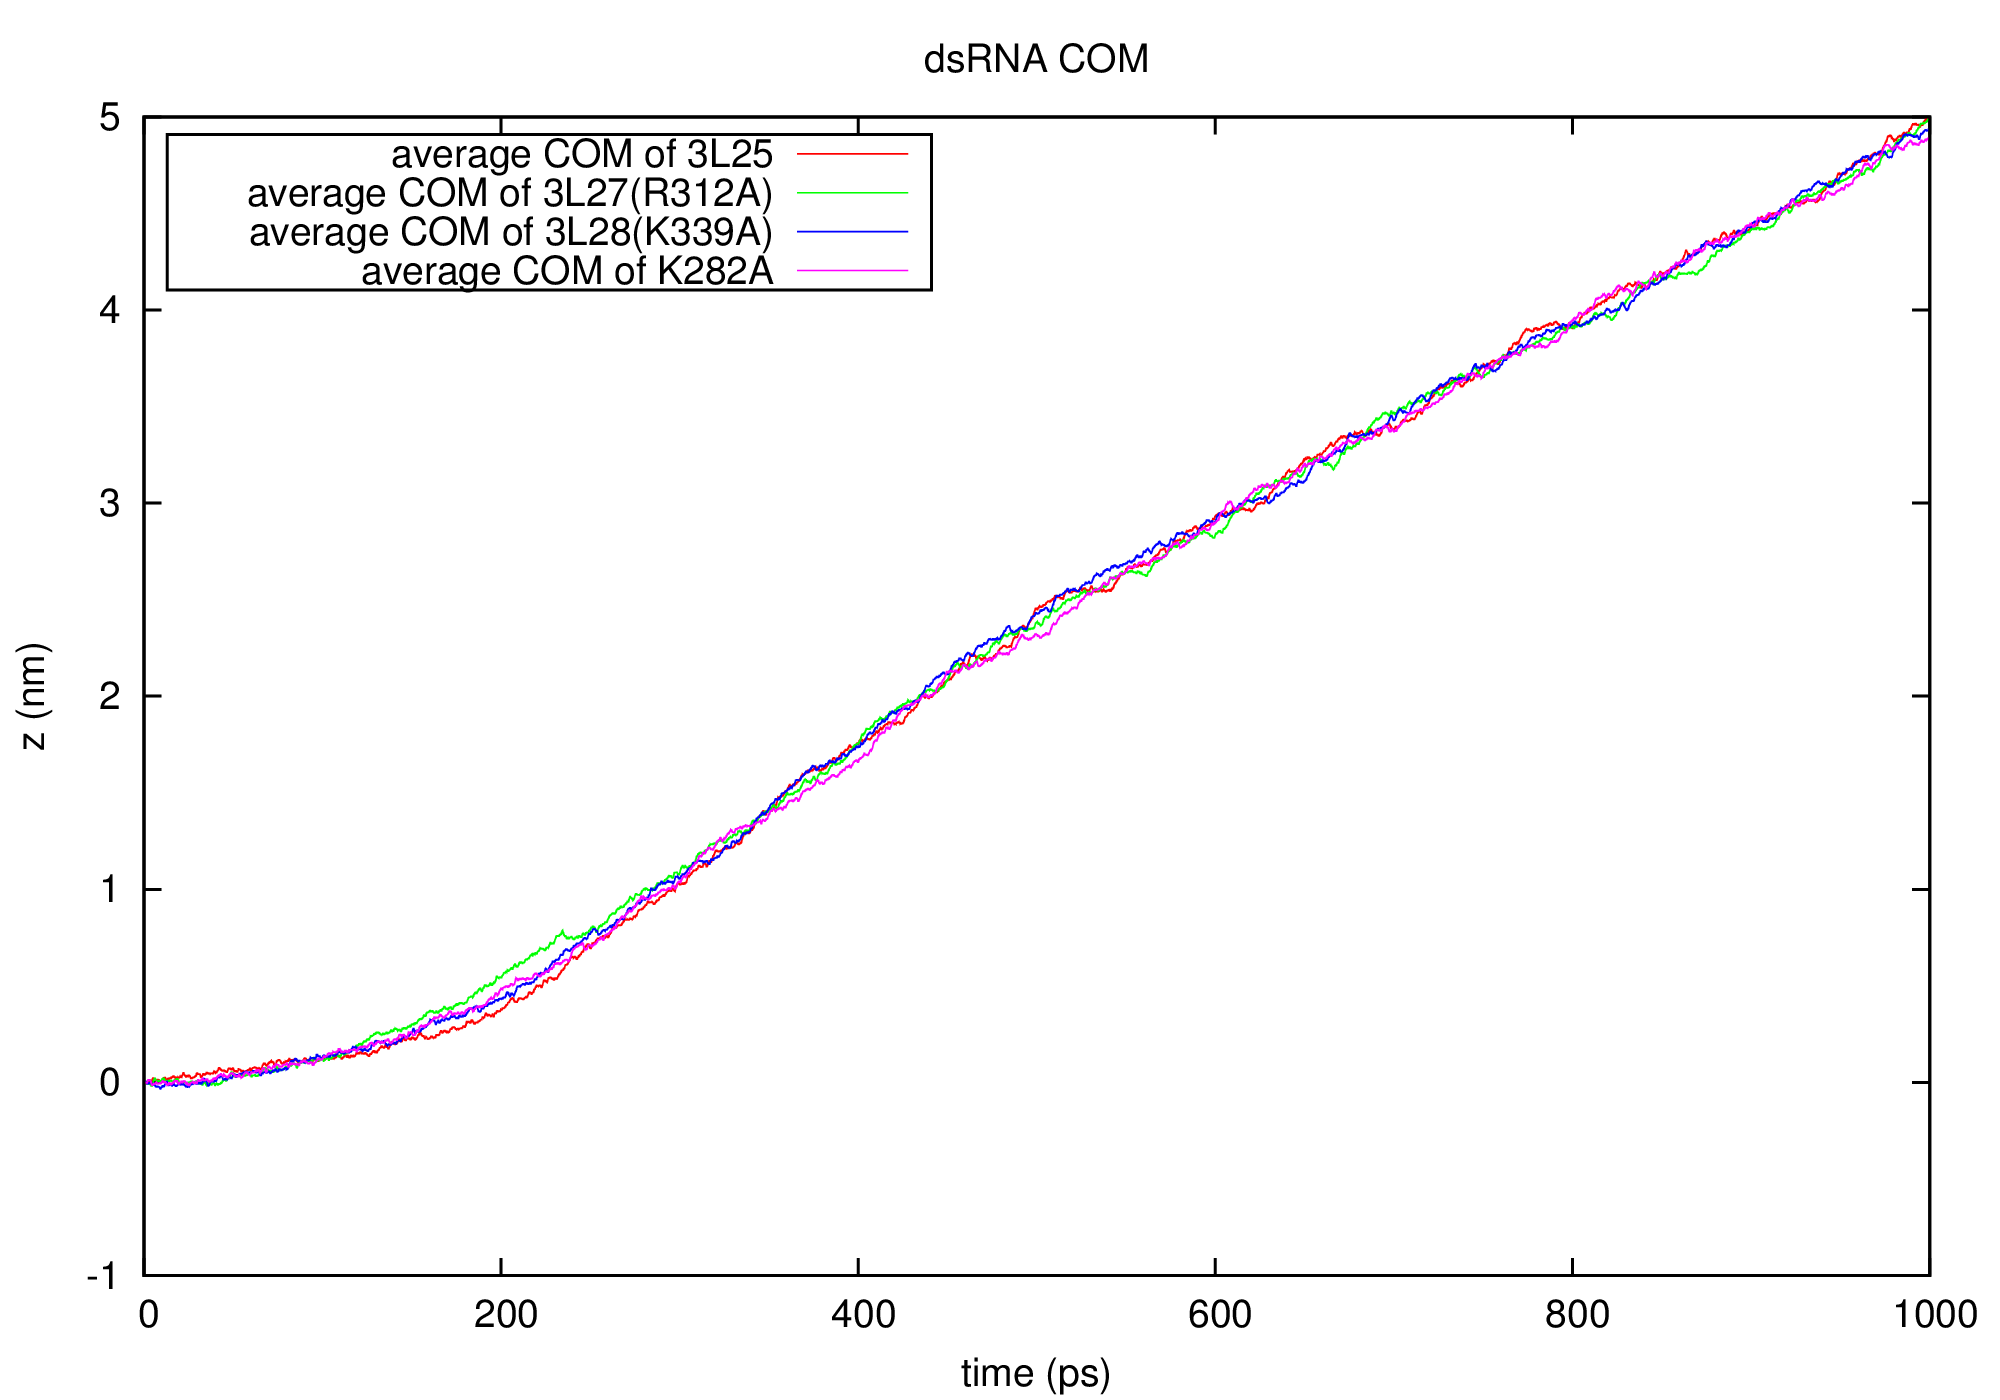
\includegraphics[width=0.7\textwidth,natwidth=610,natheight=642]{pullx}
\caption{Đường biểu diễn toạ độ khối tâm trung bình theo thời gian giữa dsRNA và VP35 với phân tử không đột biến (3L25) và đột biến (3L27, 3L28, \gls{K282A})}
\label{pullxt}
\end{figure}
Từ hình \ref{pullxt} có thể nhận thấy thời gian VP35 tương tác trực tiếp với dsRNA vào khoảng 0 đến khoảng 300 ps. Độ dốc của đồ thị từ đoạn 0 đến 200ps thấp, chứng tỏ đây là giai đoạn \gls{dsrna} tương tác với VP35 để chống lại lực kéo tách hai nhóm ra. Sau đó là giai đoạn dsRNA di chuyển với tốc độ ổn định. Điều này là hợp lý vì quá trình mô phỏng \gls{smd} sử dụng chế độ kéo với nhóm liên kết có vận tốc không đổi được trình bày ở chương trước. dsRNA được kéo ra và di chuyển đến khi không còn tương tác với VP35 nữa thì di chuyển gần như tự do.

\section{Thế năng tương tác giữa amino acid của VP35 với \glsentrytext{dsrna}}
\label{potential}
%%%%%%%%%%%%%%%%%%% Sửa "bán kính chặt cụt" bởi đoạn giải thích khác %%%%%%%%%%%%%%%%%%%%%%%%%%%%%%%%%%%%%%%%%%
Cấu hình B-conf của VP35 có 126 amino acid từ amino acid thứ 215 đến 340. Cần chọn các amino acid đáng quan tâm để thực hiện tính toán thế năng tương tác theo thời gian. Việc chọn các amino acid có khả năng tham gia liên kết với \gls{dsrna} được thực hiện như sau:
\begin{enumerate}
\item chọn phân tử bất kỳ thuộc \gls{dsrna} làm tâm
\item tất cả các amino acid của VP35 có bất kỳ phân tử nào nằm trong bán kính $r_{cutoff}=r_{Coulomb}=r_{VdW}=1.4nm$ (đã trình bày trong \ref{rcutoff}) được xem là có khả năng tương tác với \gls{dsrna}
\end{enumerate}
Kết quả của phép chọn trên được liệt kê trong phụ lục \ref{81residues}.
Quan sát 81 \gls{residue} này, có thể chọn ra các \gls{residue} tiêu biểu có khả năng đóng góp cho tương tác giữa hai nhóm phân tử này dựa trên các tiêu chí sau:
\begin{itemize}
\item Có thế năng biến đổi theo thời gian trong quá trình mô phỏng \gls{smd}. Điều này là hợp lý vì nếu \gls{residue} đó nếu thực sự đóng góp vào tương tác \gls{dsrna}--VP35 thì khi tách hai nhóm phân tử này ra, tổng thế năng tương tác của \gls{residue} này với các phân tử của \gls{dsrna} phải giảm một cách rõ rệt.
\item Độ giảm của thế năng được đánh giá dựa vào hai \gls{residue} đã được thực nghiệm xác minh tính quan trọng của nó trong tương tác \gls{dsrna}--VP35 là Arg312 và Lys339\cite{Leung2010}. Nếu độ biến thiên thế năng này có scale nhỏ hơn hẳn so với cả hai \gls{residue} trên thì đó không phải là \gls{residue} ta cần quan tâm.
\item Từ kết quả thu được, độ thay đổi thế năng của Lys339 là $10 kJ/mol$ được chọn làm giới hạn chọn lọc các amino acid cần quan tâm.
%%%%%%%%%%%%%%%%%%%%%%%%%%%%%%% Bổ sung số liệu chính xác: 10 kJ/mol %%%%%%%%%%%%%%%%%%%%%%%%%%%%%%%%%%%%%%
\end{itemize}
Từ các điều kiện trên, có thể rút ra được từ kết quả chạy mô phỏng các \gls{residue} đáng quan tâm gồm: Phe239, Glu274, Cys275, IleLE278, GLu279, Lys282, Arg312, Asp321, Arg322, Lys339, Ile340. Quan sát các đồ thị \ref{fig:Coulomb1}, \ref{fig:Coulomb2}, \ref{fig:Coulomb3}, \ref{fig:VdW} có thể thấy thời gian các amino acid tương tác với \gls{dsrna} là vào khoảng 200ps đầu tiên, kể từ 400ps trở về sau thế năng tương tác giữa các amino acid và \gls{dsrna} giảm về 0. Điều này phù hợp với kết quả quan sát \ref{distance}.

Các đồ thị trong hình \ref{fig:Coulomb1}, \ref{fig:Coulomb2}, \ref{fig:Coulomb3}, \ref{fig:VdW} lấy dữ liệu từ lần mô phỏng \gls{smd} thứ 2 đối với cấu hình 3L25 (tức cấu hình không đột biến). Dữ liệu từ lần mô phỏng \gls{smd} thứ 1 và thứ 3 cũng cho kết quả tương tự.

%%%%%%%%%%%%%%%%%%%%%%%%% print riêng lẻ từng hình để có độ phân giải cao, remove English caption, notation %%%%%%%%%%%%%%%%%%%%%%%%%%%%

\begin{figure}[h!]
\begin{subfigure}{\textwidth}
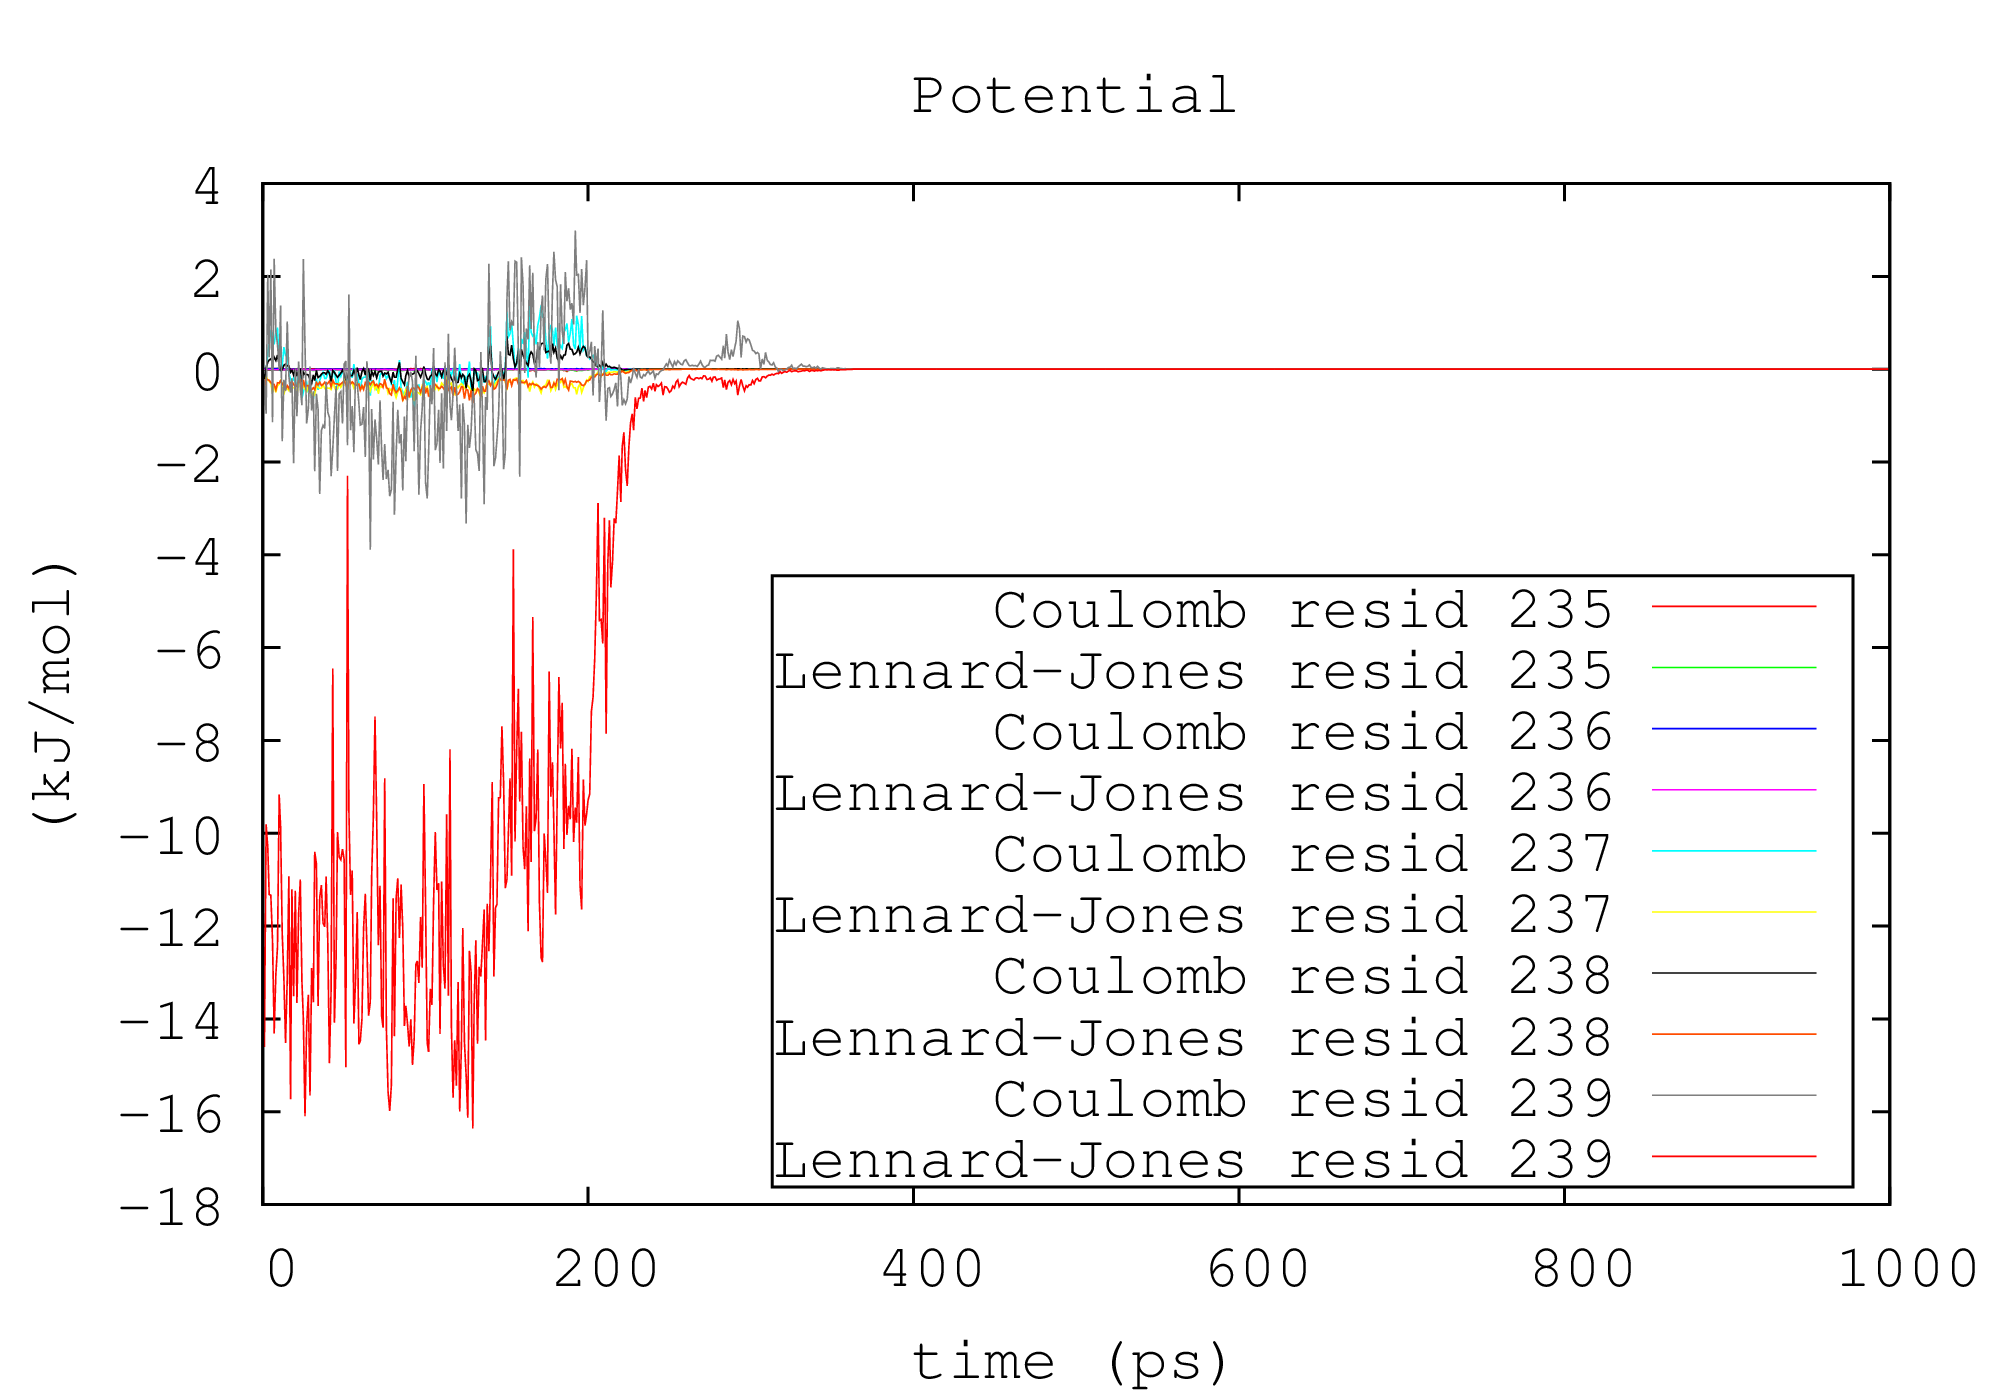
\includegraphics[width=0.9\textwidth,natwidth=610,natheight=642]{235-239}
\caption{\gls{residue} 235--239, tiêu biểu Phe239}
\label{fig:239}
\end{subfigure}\\
\begin{subfigure}{\textwidth}
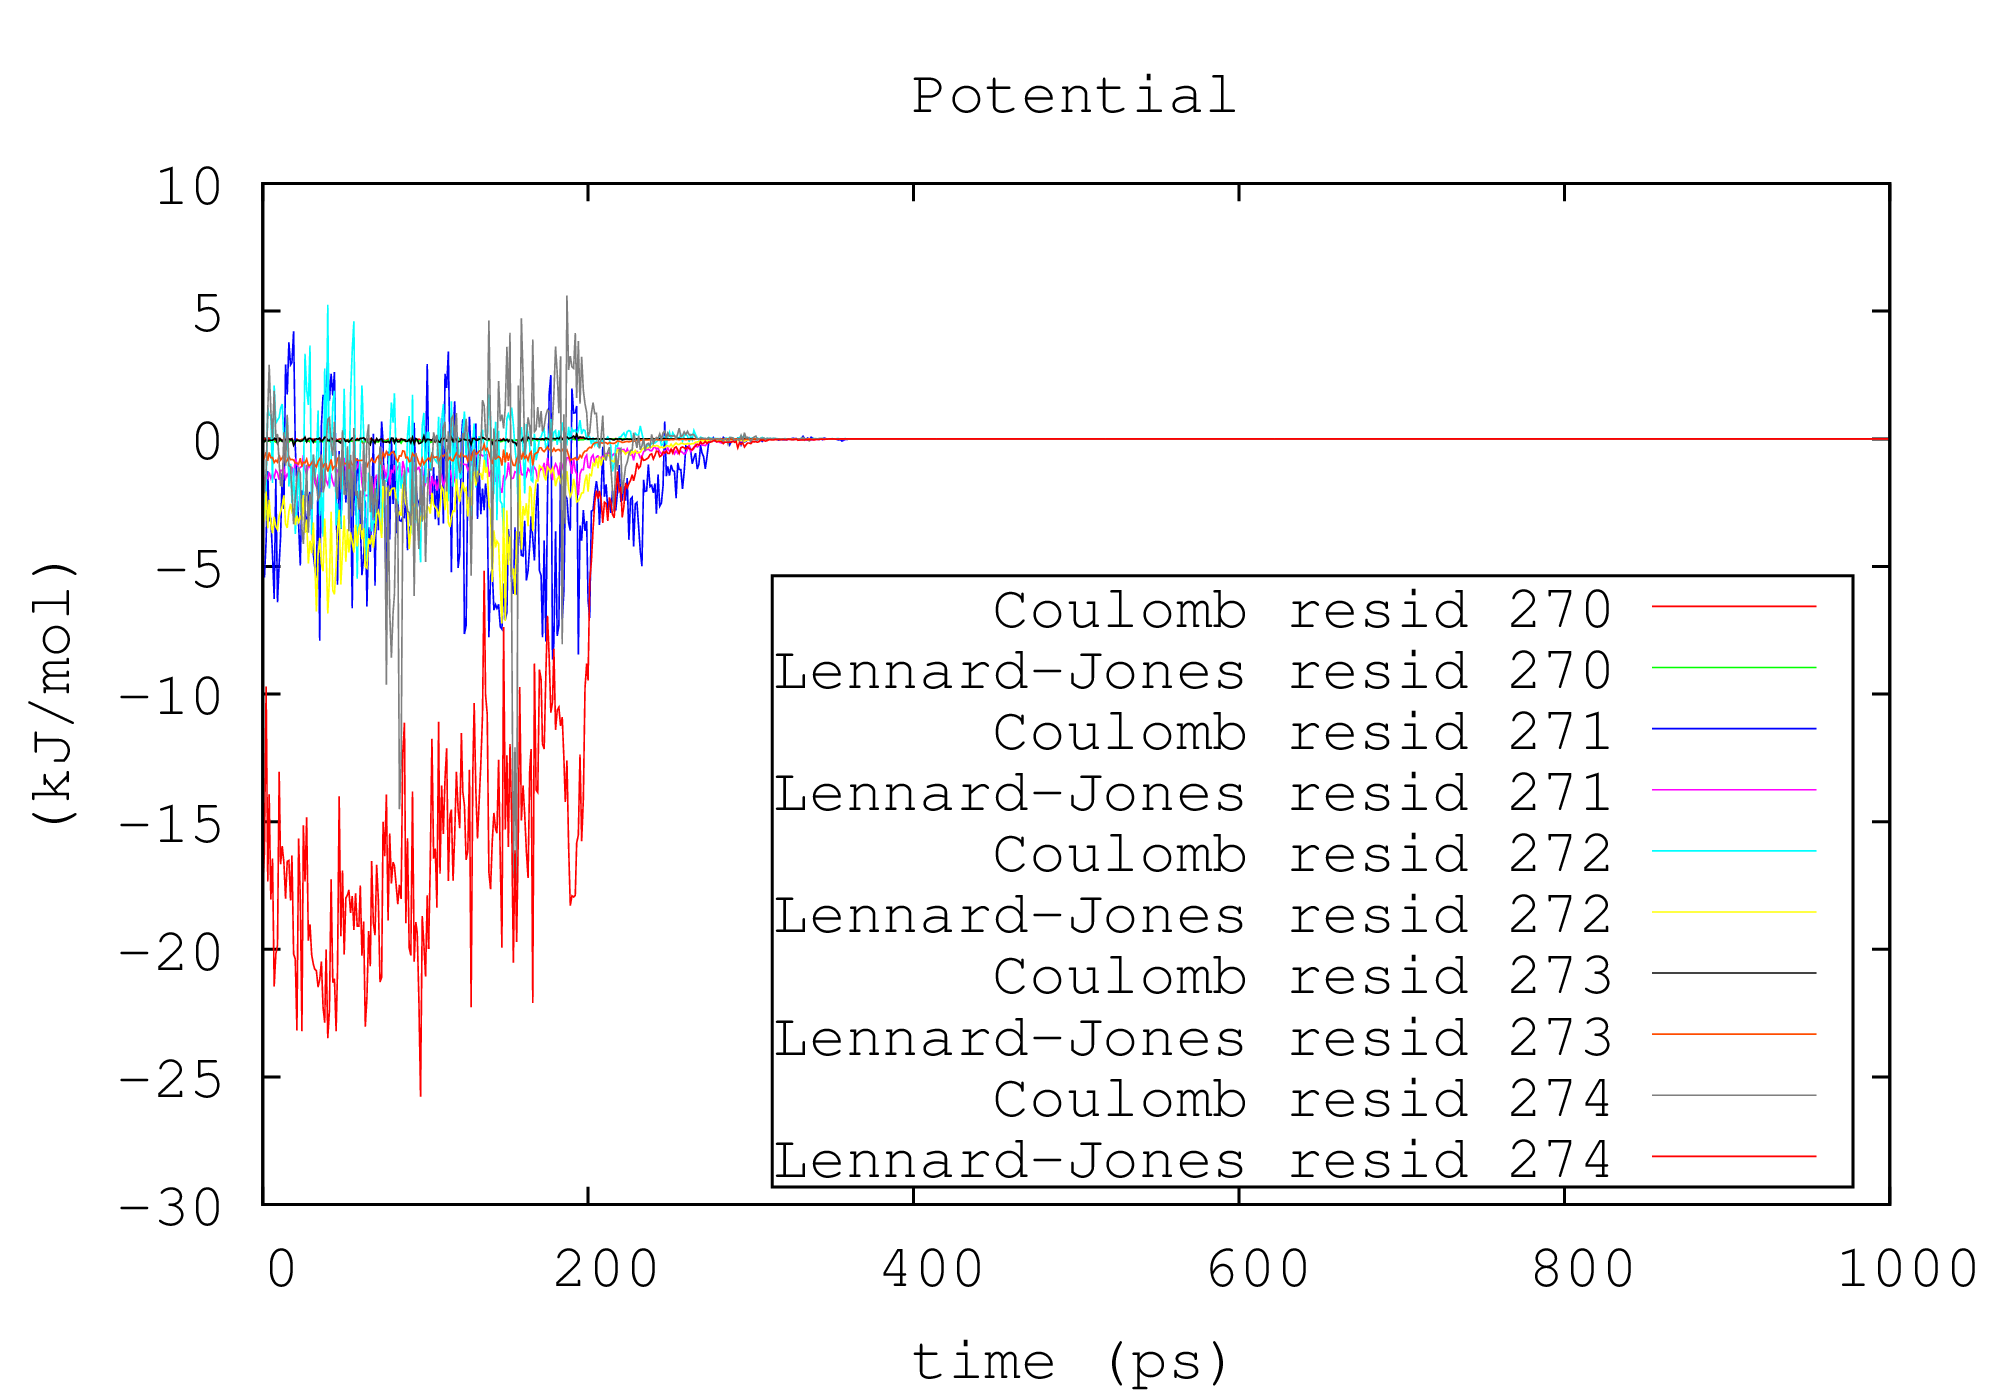
\includegraphics[width=0.9\textwidth,natwidth=610,natheight=642]{270-274}
\caption{\gls{residue} 270--274, tiêu biểu Q274}
\label{fig:274}
\end{subfigure}
\caption{Đồ thị thế năng theo thời gian của các amino acid}
\label{fig:Coulomb1}
\end{figure}
\begin{figure}[h!]
\begin{subfigure}{\textwidth}
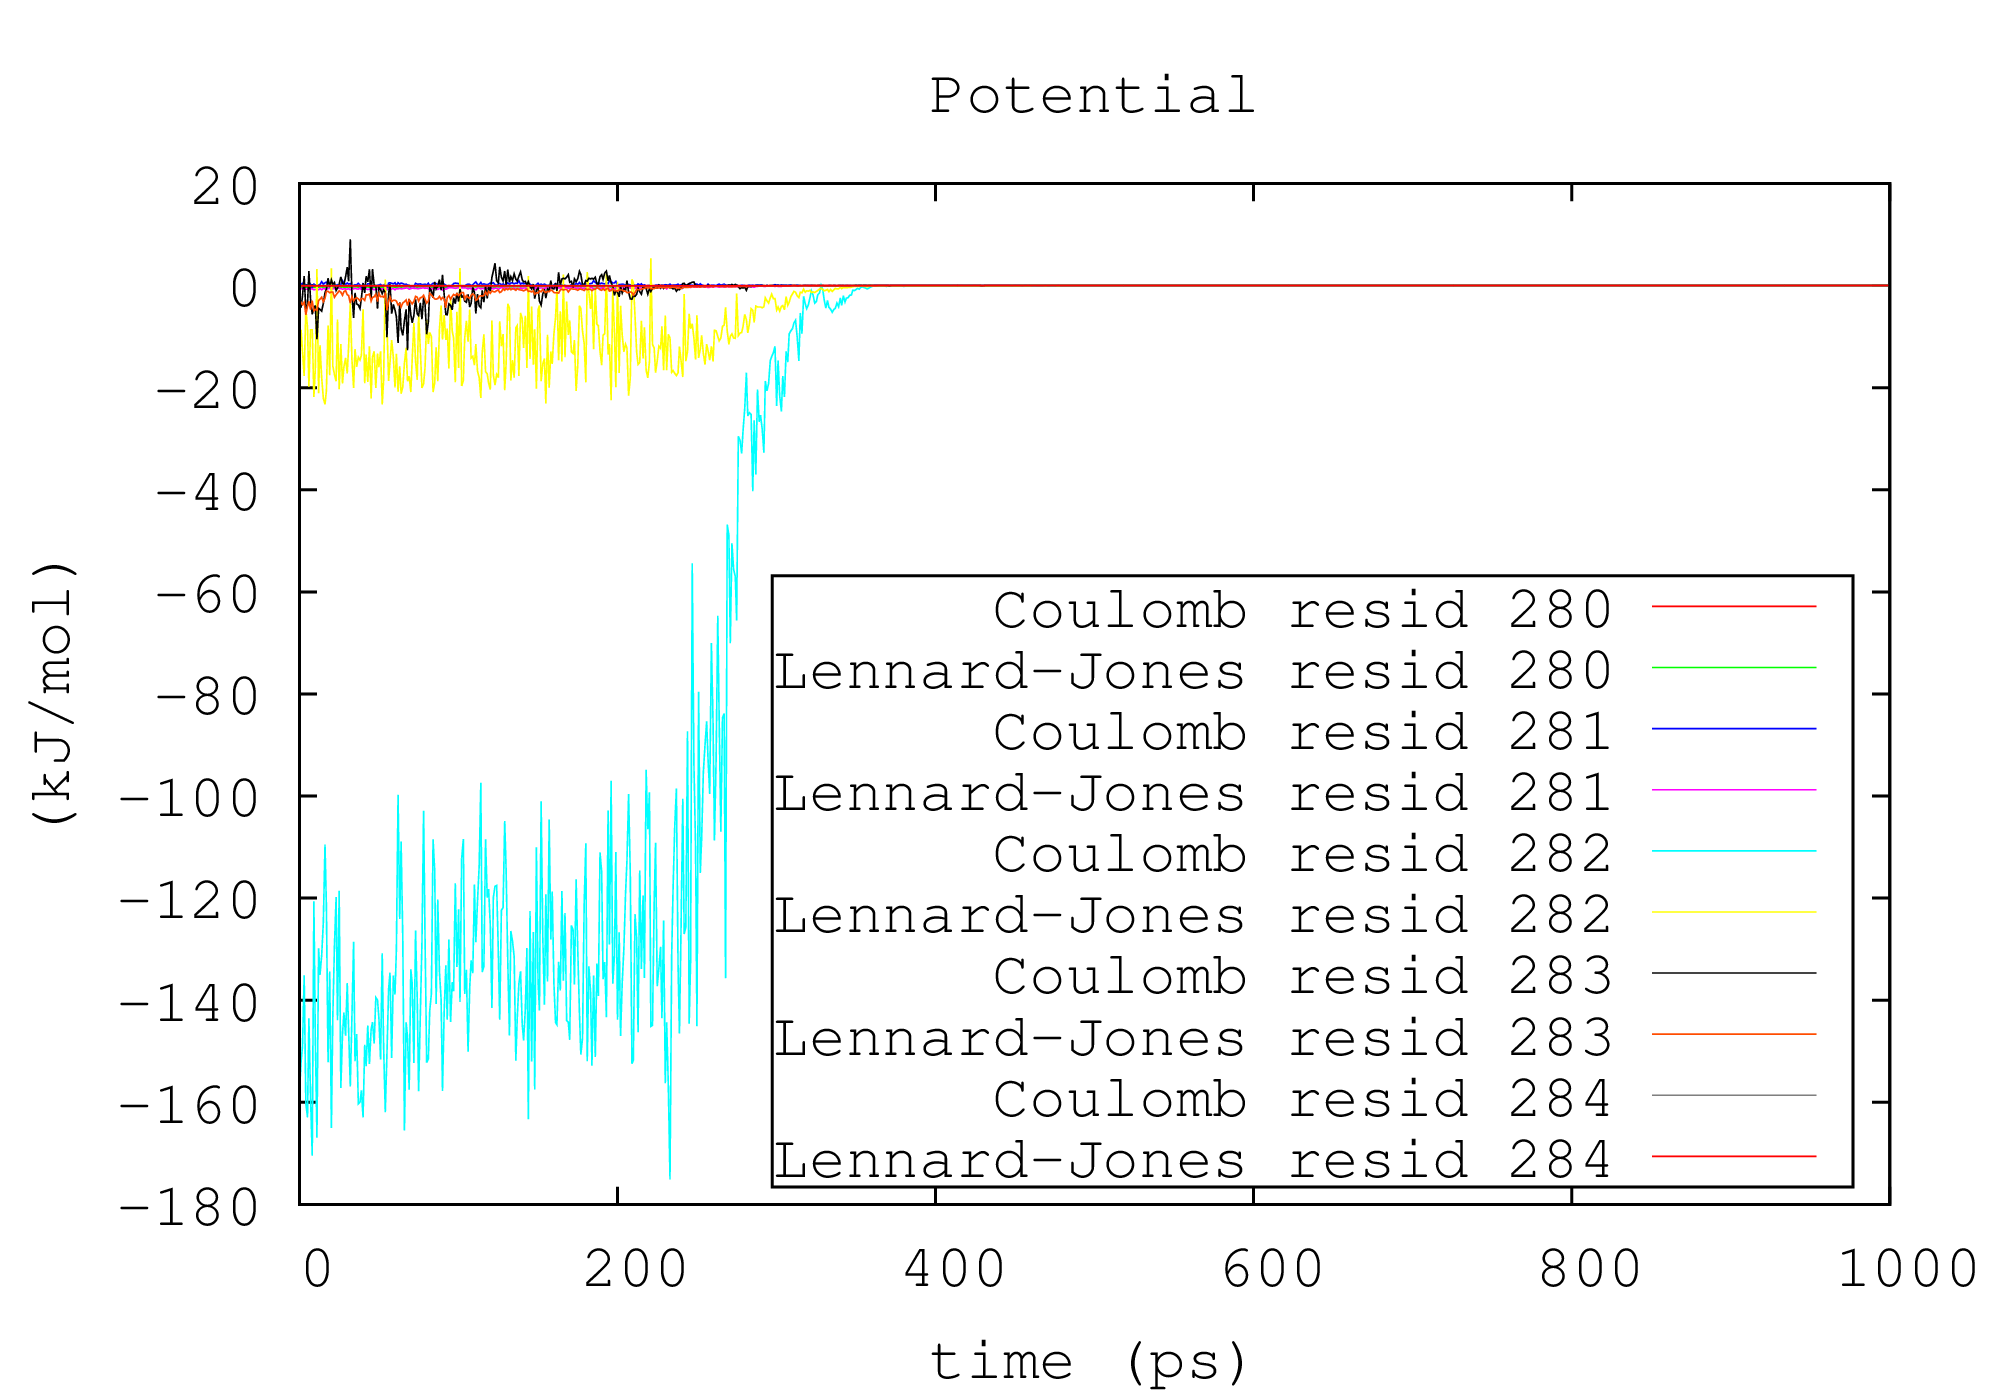
\includegraphics[width=0.9\textwidth,natwidth=610,natheight=642]{280-284}
\caption{\gls{residue} 280--284, tiêu biểu Lys282}
\label{fig:282}
\end{subfigure}\\
\begin{subfigure}{\textwidth}
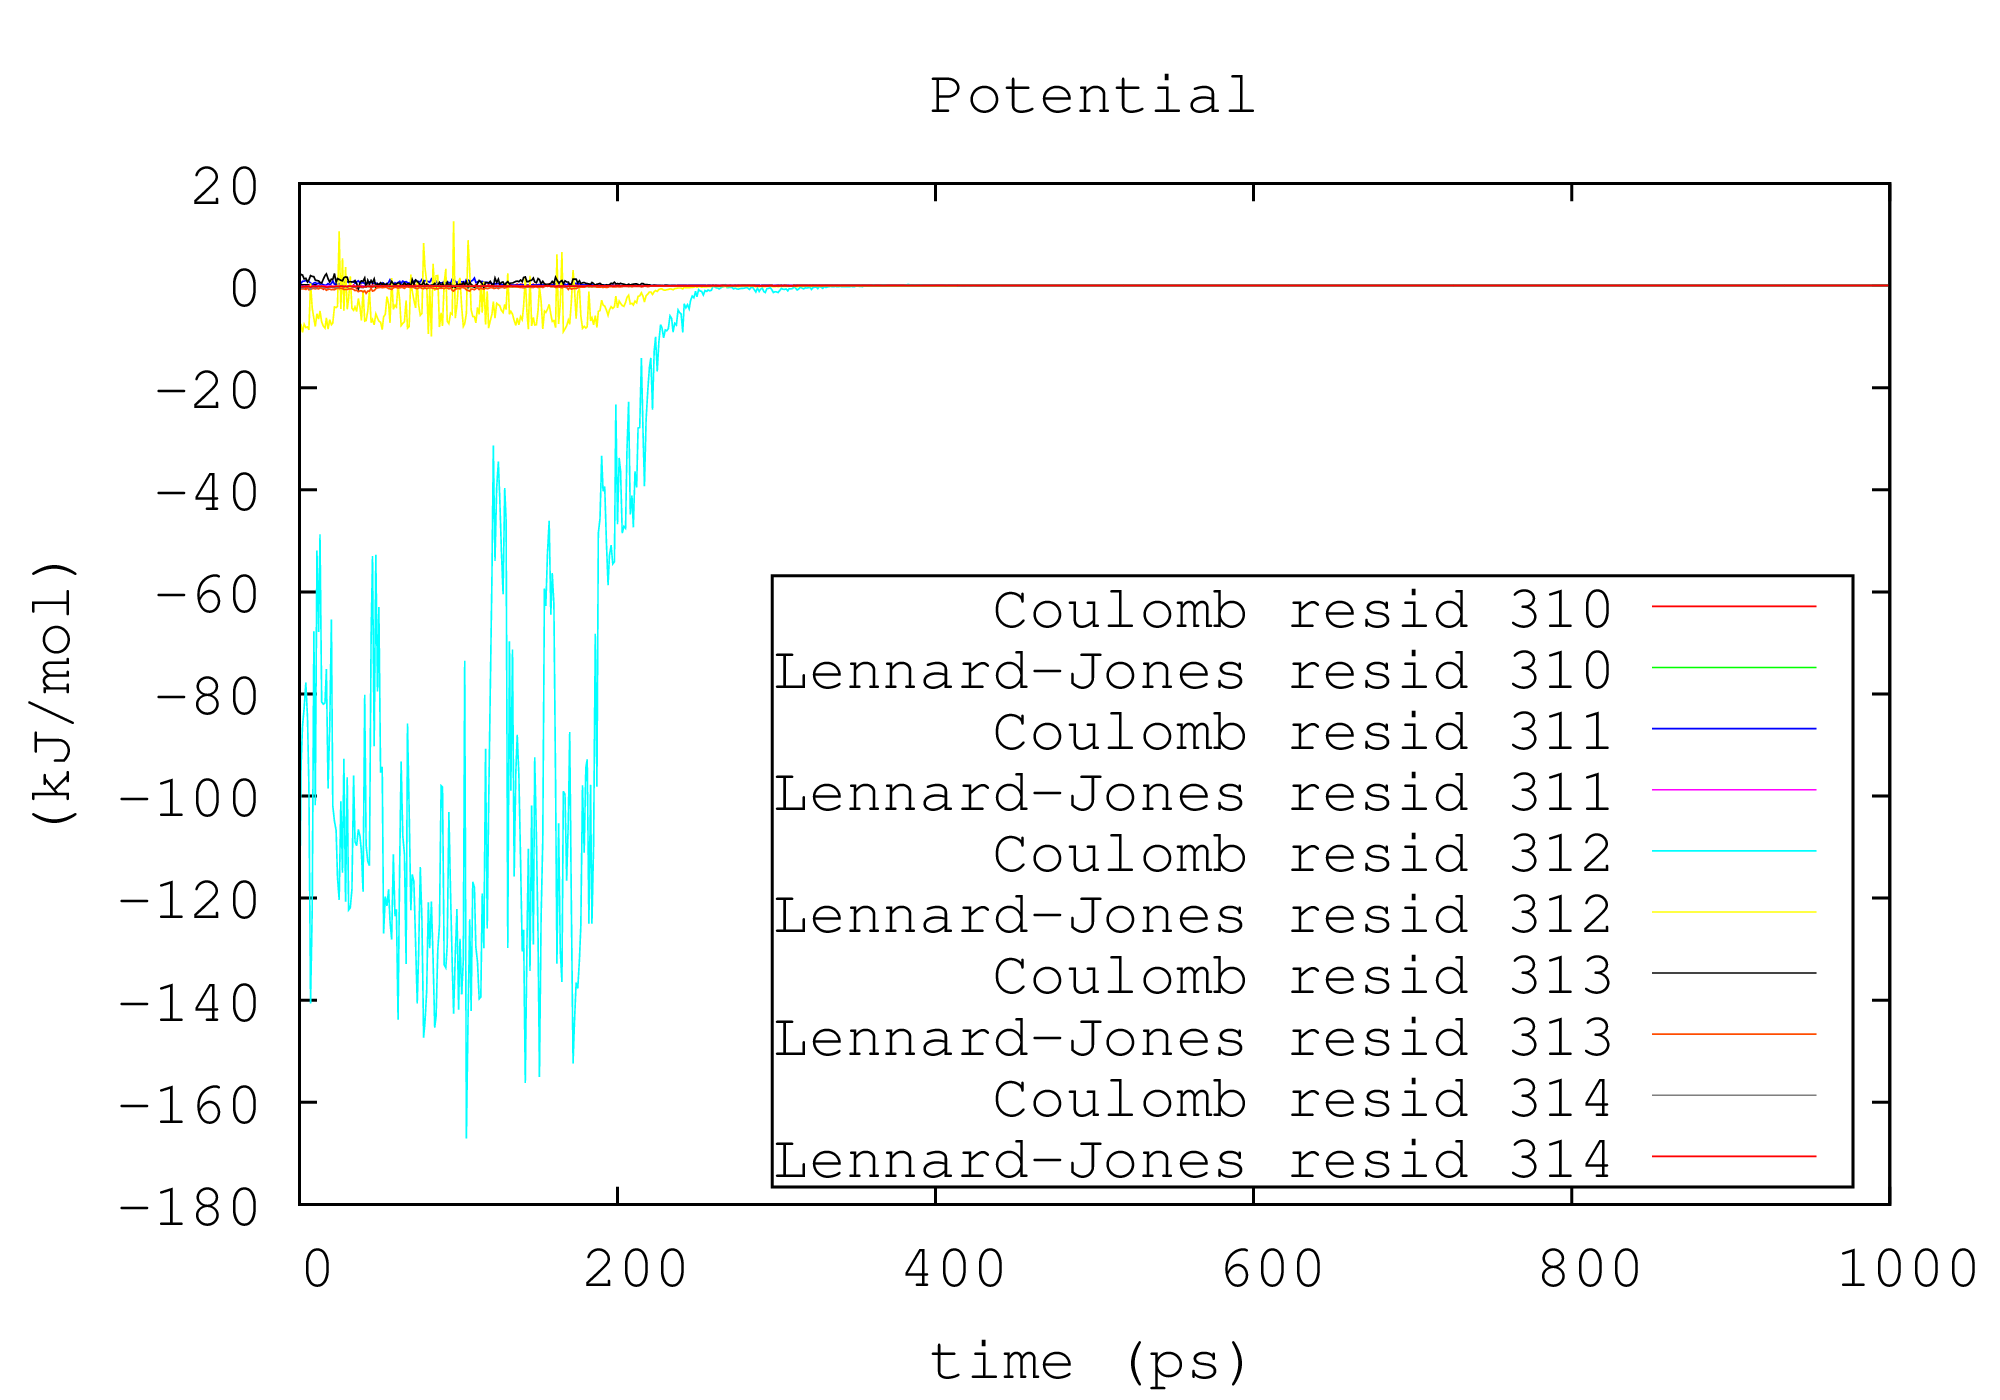
\includegraphics[width=0.9\textwidth,natwidth=610,natheight=642]{310-314}
\caption{\gls{residue} 310-314, tiêu biểu Arg312 (khoảng 120 kJ/mol)}
\label{fig:312}
\end{subfigure}
\caption{Đồ thị thế năng theo thời gian của các amino acid}
\label{fig:Coulomb2}
\end{figure}
\begin{figure}[h!]
\begin{subfigure}{\textwidth}
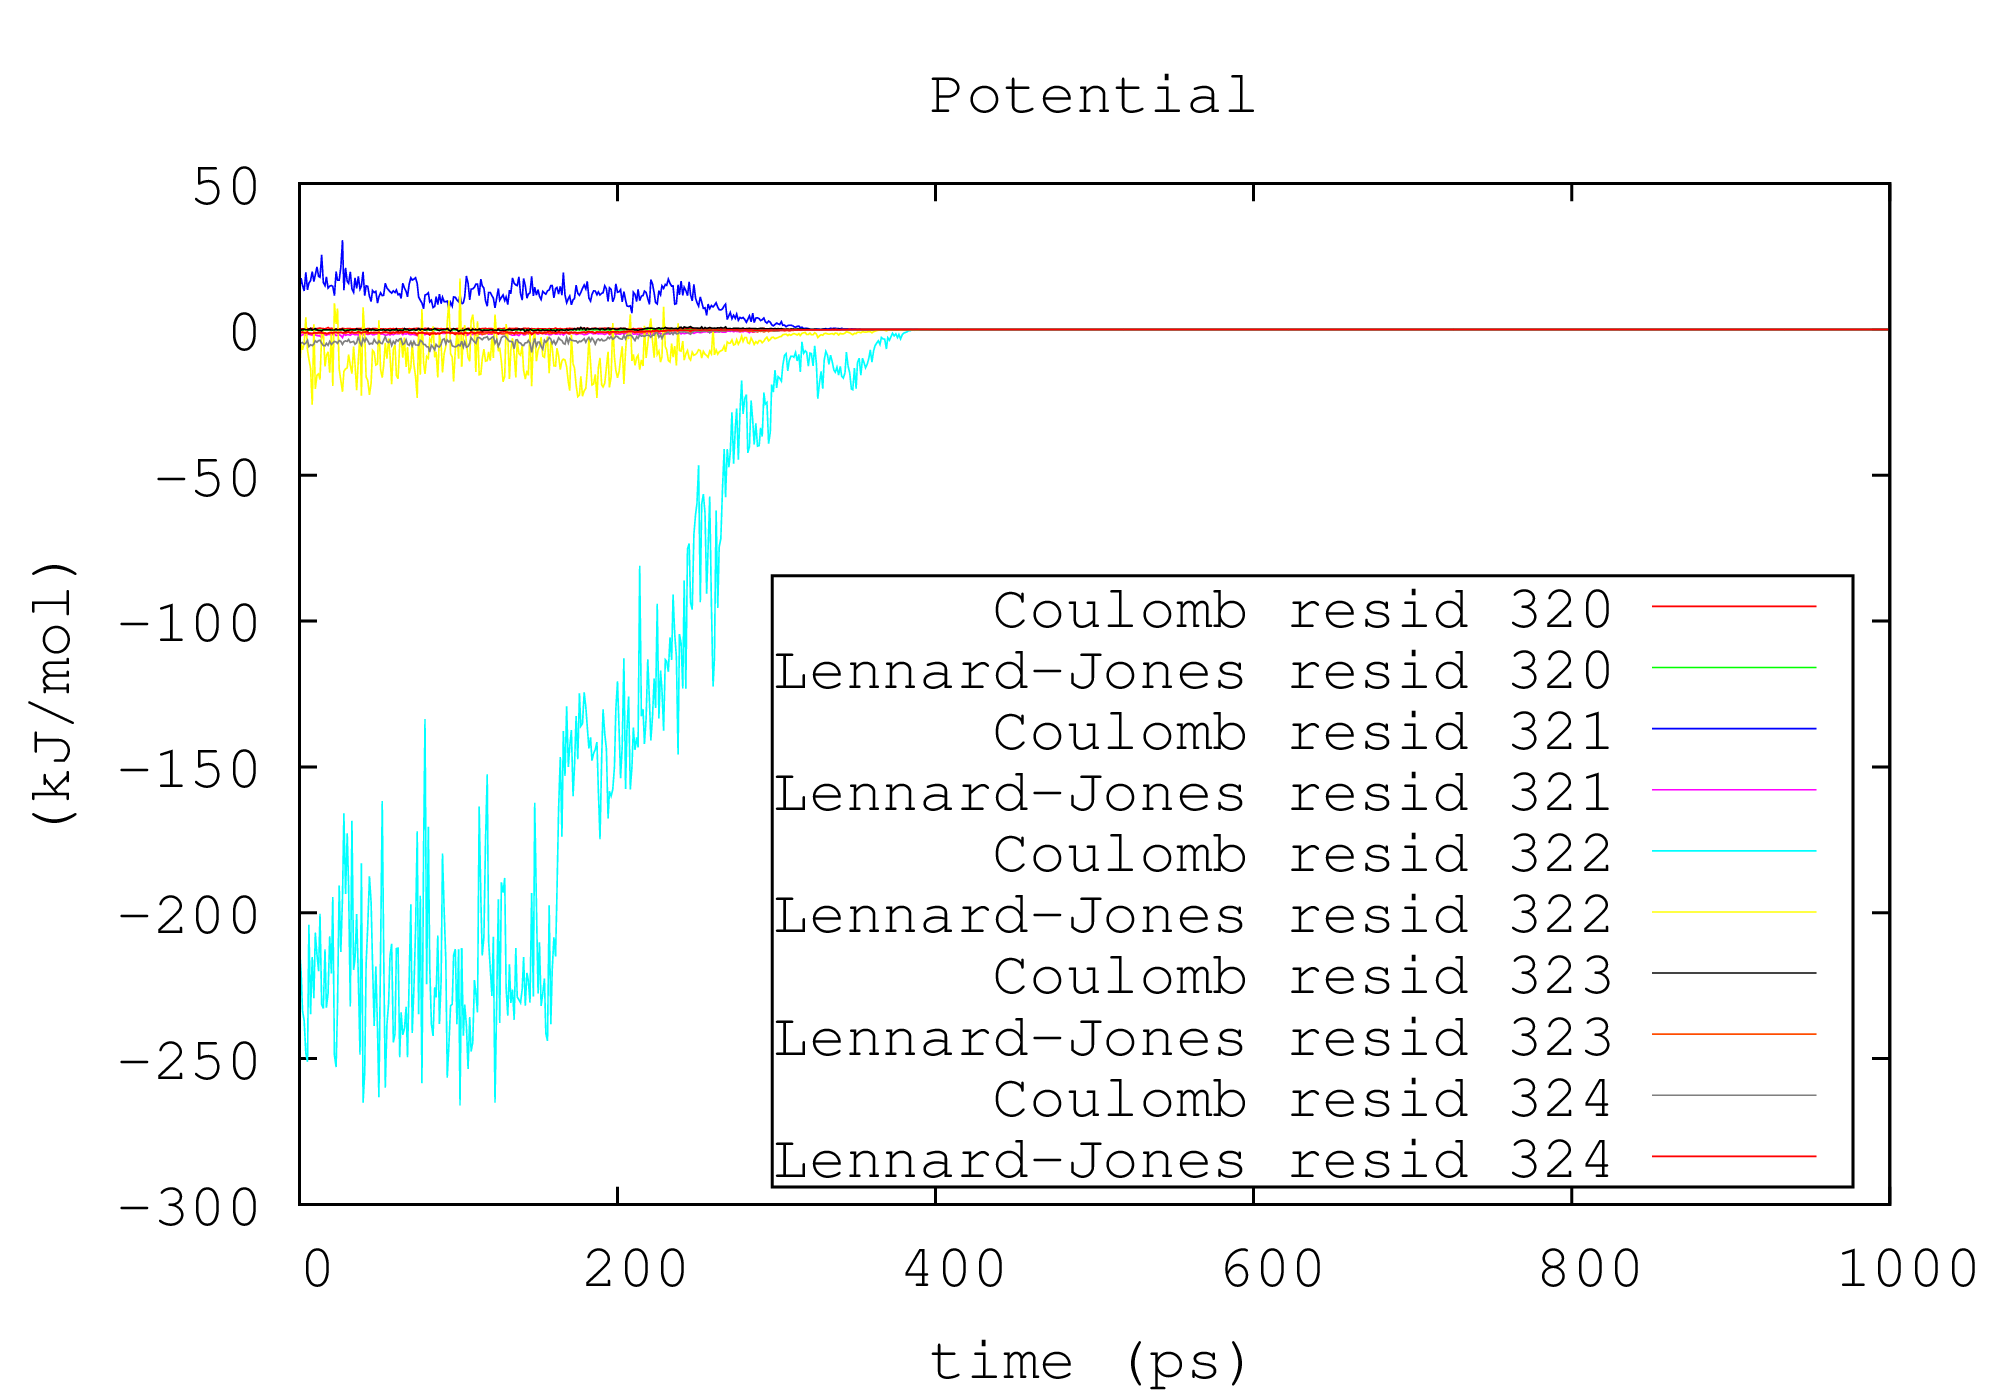
\includegraphics[width=0.9\textwidth,natwidth=610,natheight=642]{320-324}
\caption{\gls{residue} 320--324, tiêu biểu Asp321, Arg322}
\label{fig:322}
\end{subfigure}\\
\begin{subfigure}{\textwidth}
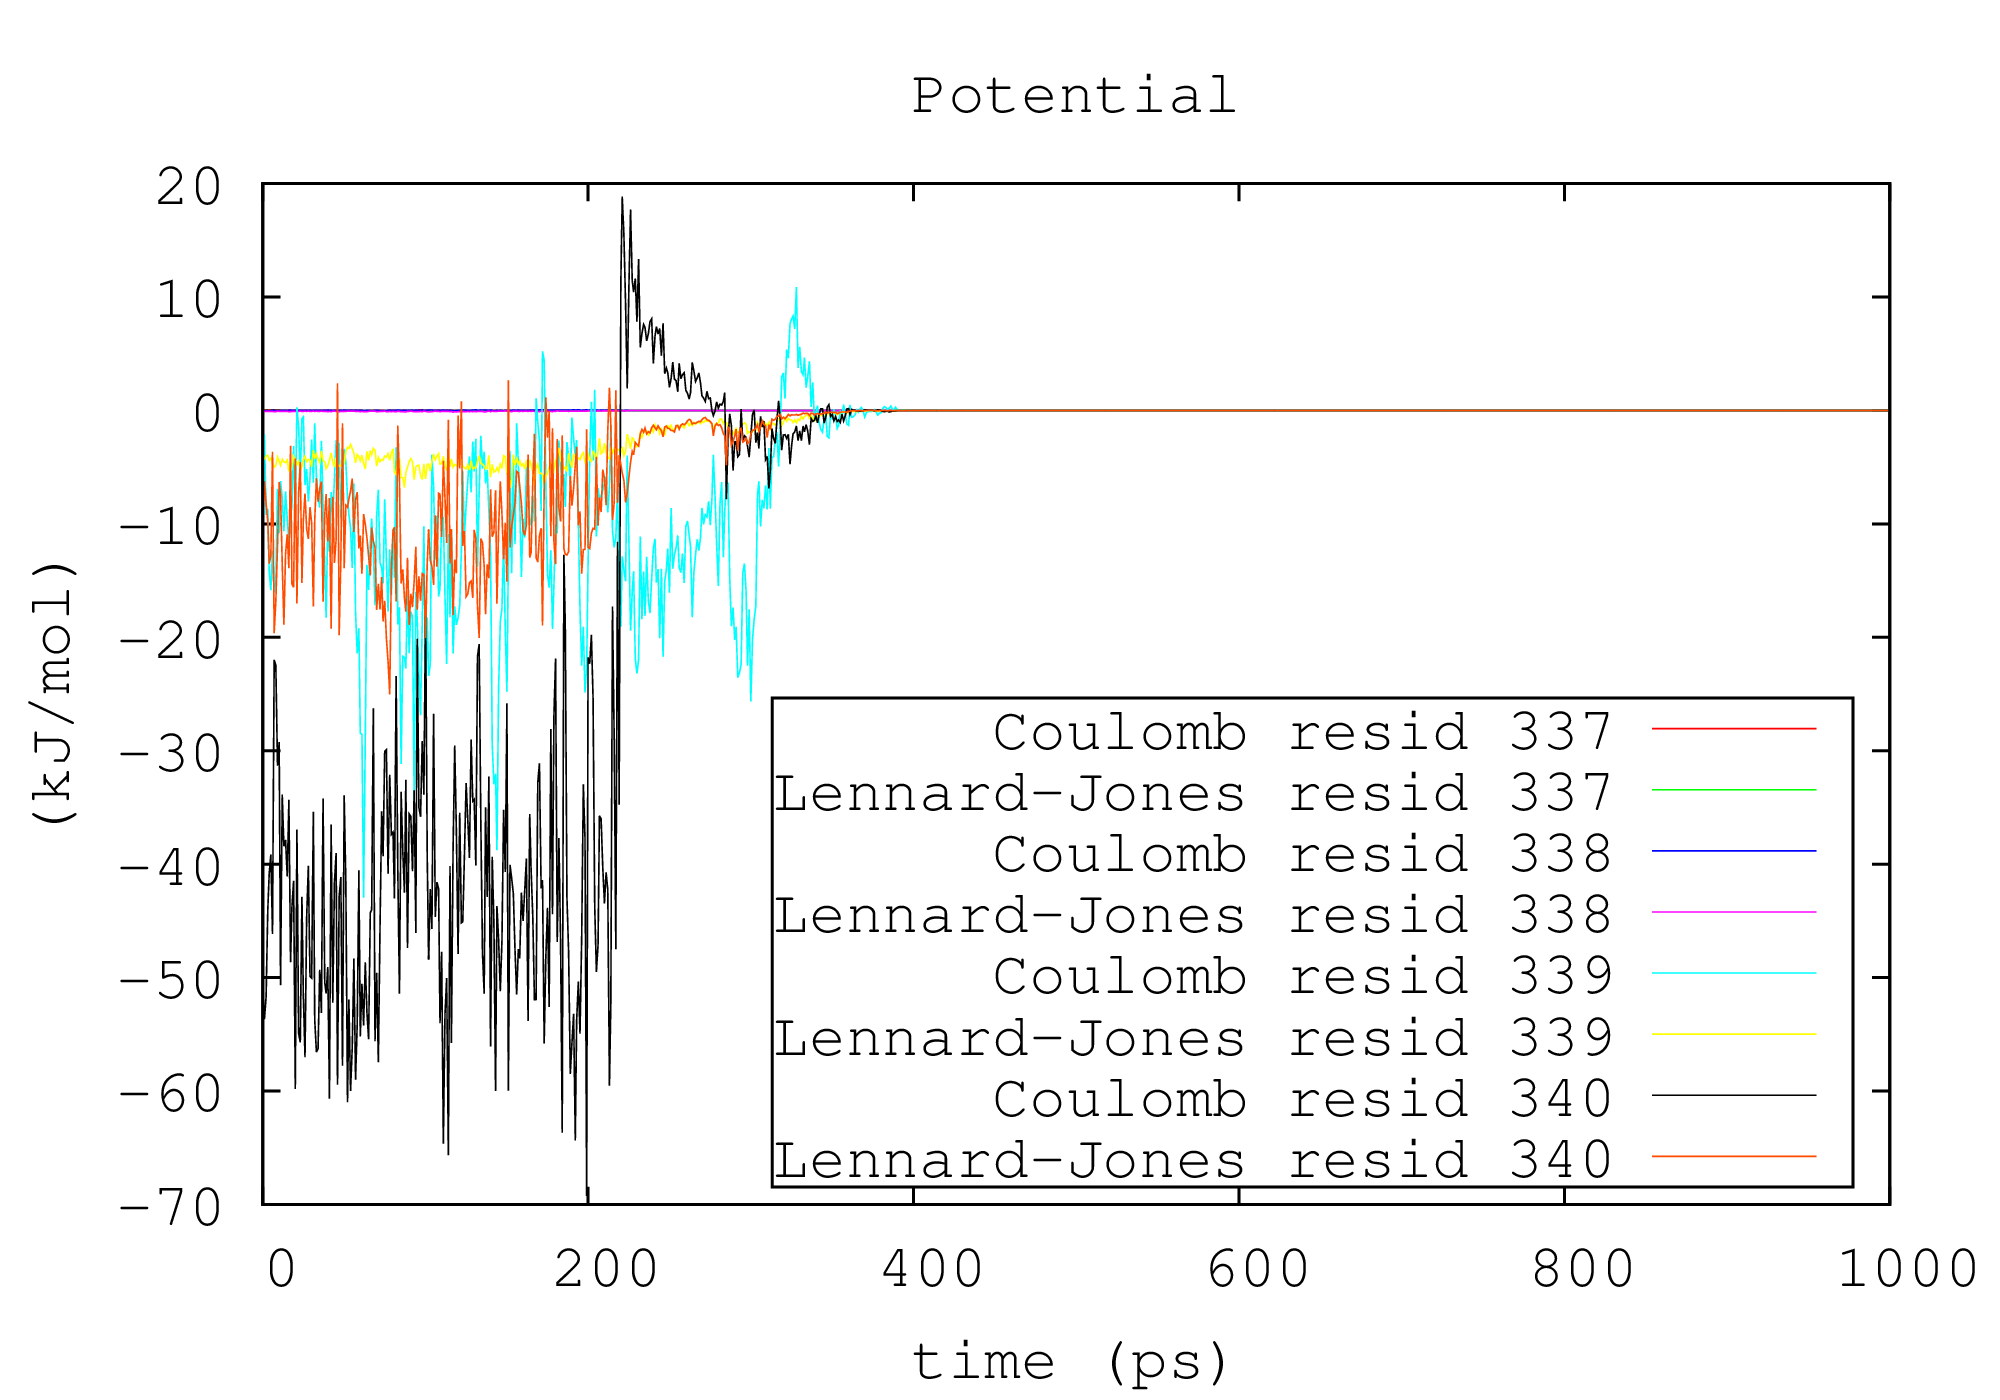
\includegraphics[width=0.9\textwidth,natwidth=610,natheight=642]{337-340}
\caption{\gls{residue} 337--340, tiêu biểu  ILE340, Lys339 (khoảng 10--20 kJ/mol)}
\label{fig:339}
\end{subfigure}
\caption{Đồ thị thế năng theo thời gian của các amino acid}
\label{fig:Coulomb3}
\end{figure}
\begin{figure}[h]
\begin{center}
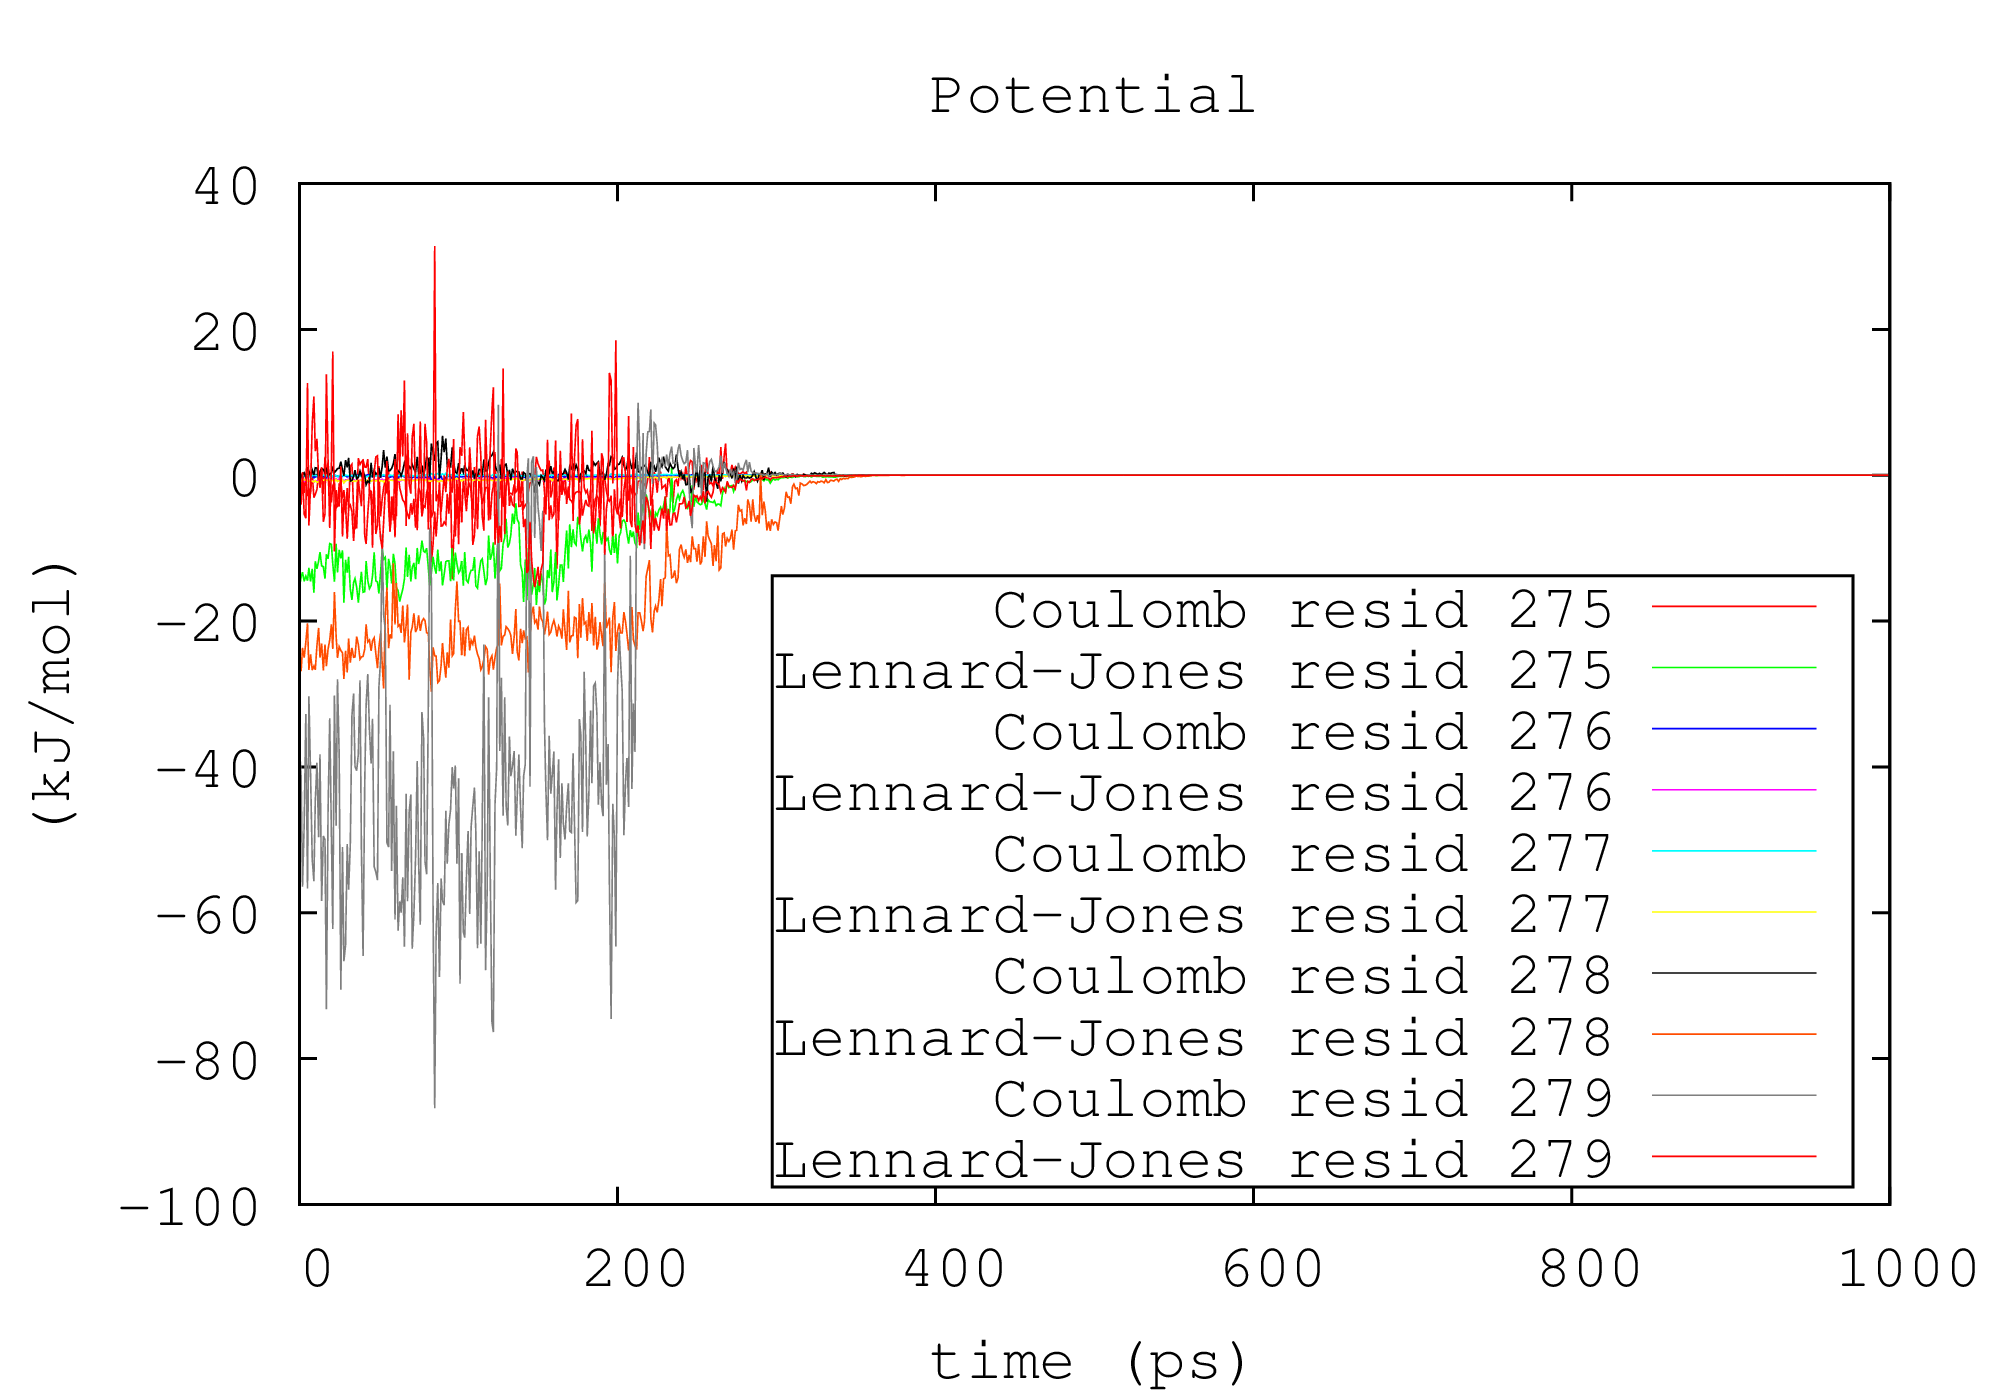
\includegraphics[width=1.0\textwidth,natwidth=610,natheight=642]{275-279}
\end{center}
\caption{\gls{residue} 275--279, tiêu biểu Cys275, Ile278, Glu279. Glu279 tương tác Coulomb là chủ yếu. Cys275, Ile278 tương tác VdW là chủ yếu với thế năng cùng scale với thế năng của Lys339.}
\label{fig:VdW}
\end{figure}
Dựa vào đồ thị \ref{fig:Coulomb1},\ref{fig:Coulomb2},\ref{fig:Coulomb3}, có thể thấy rằng đóng góp của tương tác Coulomb là rất đáng kể. Tuy nhiên vẫn có những \gls{residue} có đóng góp của tương tác Van der Waals là đáng kể, đó là Cys275 và Ile278 (xem đồ thị \ref{fig:VdW}).

Dựa vào đồ thị \ref{fig:339} và \ref{fig:312} có thể thấy Arg312 đóng vai trò tương tác trực tiếp với \gls{dsrna}. Mặc dù đột biến \gls{K339A} cũng gây mất liên kết \gls{dsrna}--VP35 trong thực nghiệm, nhưng độ thay đổi thế năng tương tác do Lys339 gây ra không nhiều, chỉ khoảng $10\%$ khi so với Arg312 gây ra. Ngoài ra, Lys282 và Arg322 cũng tương tác nhiều với \gls{dsrna} do thế năng tương tác giữa các \gls{residue} này với \gls{dsrna} lớn (Lys282 có thế năng tương tác lên hơn $140 kJ/mol$, Arg322 có thế năng tương tác lên đến $250 kJ/mol$, Arg312 có thế năng tương tác chỉ ở mức $140 kJ/mol$). Xem hình \ref{fig:282}, \ref{fig:312}, \ref{fig:322}. Các amino acid này có thể đóng vai trò quan trọng trong tương tác giữa \gls{dsrna}--VP35.
%\clearpage

\section{Kết quả phân tích liên kết Hydro giữa các amino acid của VP35 với \glsentrytext{dsrna}}
\label{hbond-result}
\begin{figure}[h!]
%\vspace{-20pt}
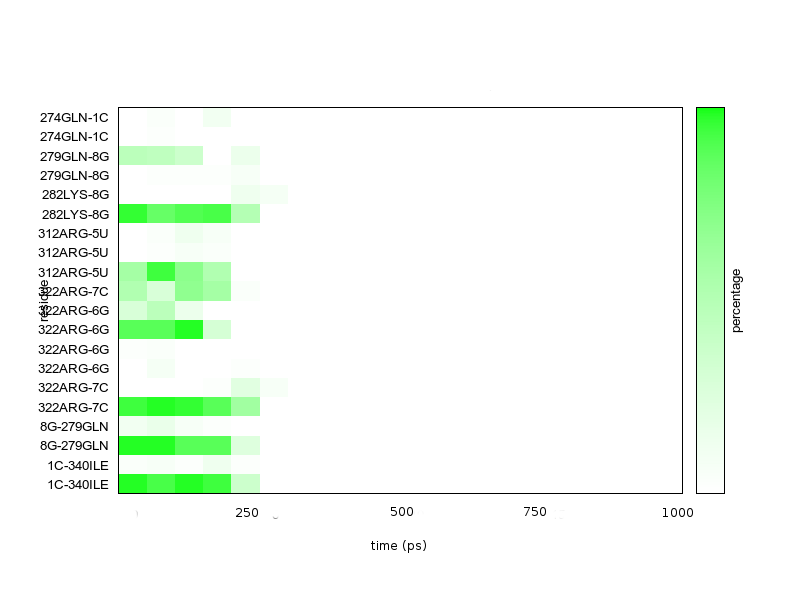
\includegraphics[width=\textwidth,natwidth=610,natheight=642]{hbond3L25_pull2}
%\vspace{-40pt}
\caption{Liên kết Hydro theo thời gian giữa các \gls{residue} và \gls{dsrna}. Lần kéo thứ 2 cấu hình B-conf của phân tử có PDBID: 3L25.}
\label{fig:hbond3L25_pull2}
\end{figure}

Hình \ref{fig:hbond3L25_pull2} cho thấy kết quả phân tích liên kết Hydro theo thời gian. Số \gls{residue} tham gia tạo liên kết Hydro không nhiều nên từ kết quả này có thể sàng lọc ra các \gls{residue} hiệu quả hơn. Đây là kết quả từ lần kéo thứ 2 cấu hình B-conf của 3L25. Các lần kéo khác cũng có kết quả tương tự. Xem phụ lục \ref{hbond}.

Phân tích kết quả thu được trong cả ba lần kéo, dễ dàng nhận thấy các \gls{residue} có khả năng đóng vai trò chủ yếu trong tương tác trực tiếp giữa \gls{dsrna}--VP35 gồm Q274, Glu279, Lys282, Arg312, Arg322, I340.

Cụ thể, các \gls{residue} nổi bật với tỉ lệ tạo liên kết Hydro cao (màu xanh đậm trên hình \ref{fig:hbond3L25_pull2}) gồm Lys282, Arg312, Arg322, Glu279 và Ile340. Ile340 là amino acid ở C-terminal nên dù có nhánh bên kỵ nước nhưng gốc $\text{OH}^{-}$ của mạch chính vẫn có khả năng tạo liên kết Hydro. Xem hình \ref{fig:Ile340}. Các amino acid này có thể đóng vai trò quan trọng trong tương tác giữa \gls{dsrna}--VP35.
\begin{figure}[h]
\centering
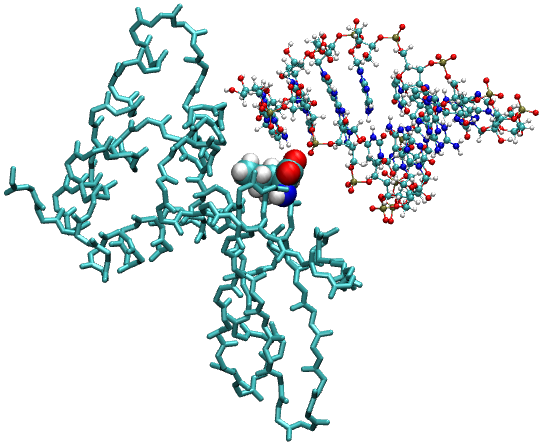
\includegraphics[width=0.7\textwidth,natwidth=610,natheight=642]{ILE340}
\caption{Mạch chính (Backbone) của VP35 được tô màu xanh da trời. Amino acid Ile340 nằm tại C-terminal nên là amino acid cuối cùng, có gốc $\text{OH}^{-}$ có khả năng tạo liên kết Hydro với \gls{dsrna}. Nguyên tử Oxy được tô màu đỏ.}
\label{fig:Ile340}
\end{figure}

\section{So sánh lực kéo}

Quan sát hình \ref{pullft} dễ dàng nhận thấy rằng lực kéo tối đa dùng để tách dsRNA với phân tử không đột biến VP35 là lớn nhất. Điều này phù hợp với kết quả thực nghiệm\cite{Leung2010}. Cũng từ kết quả thu được, lực kéo tối đa dùng để kéo phân tử VP35 đột biến tại Arg312 (\gls{R312A} - cấu hình 3L27) thấp hơn hẳn so với lực kéo phân tử không đột biến, điều này cho thấy tầm quan trọng của amino acid tại vị trí này trong tương tác dsRNA-VP35.
	\begin{figure}[t!]
	\centering
	\begin{subfigure}{0.95\textwidth}
	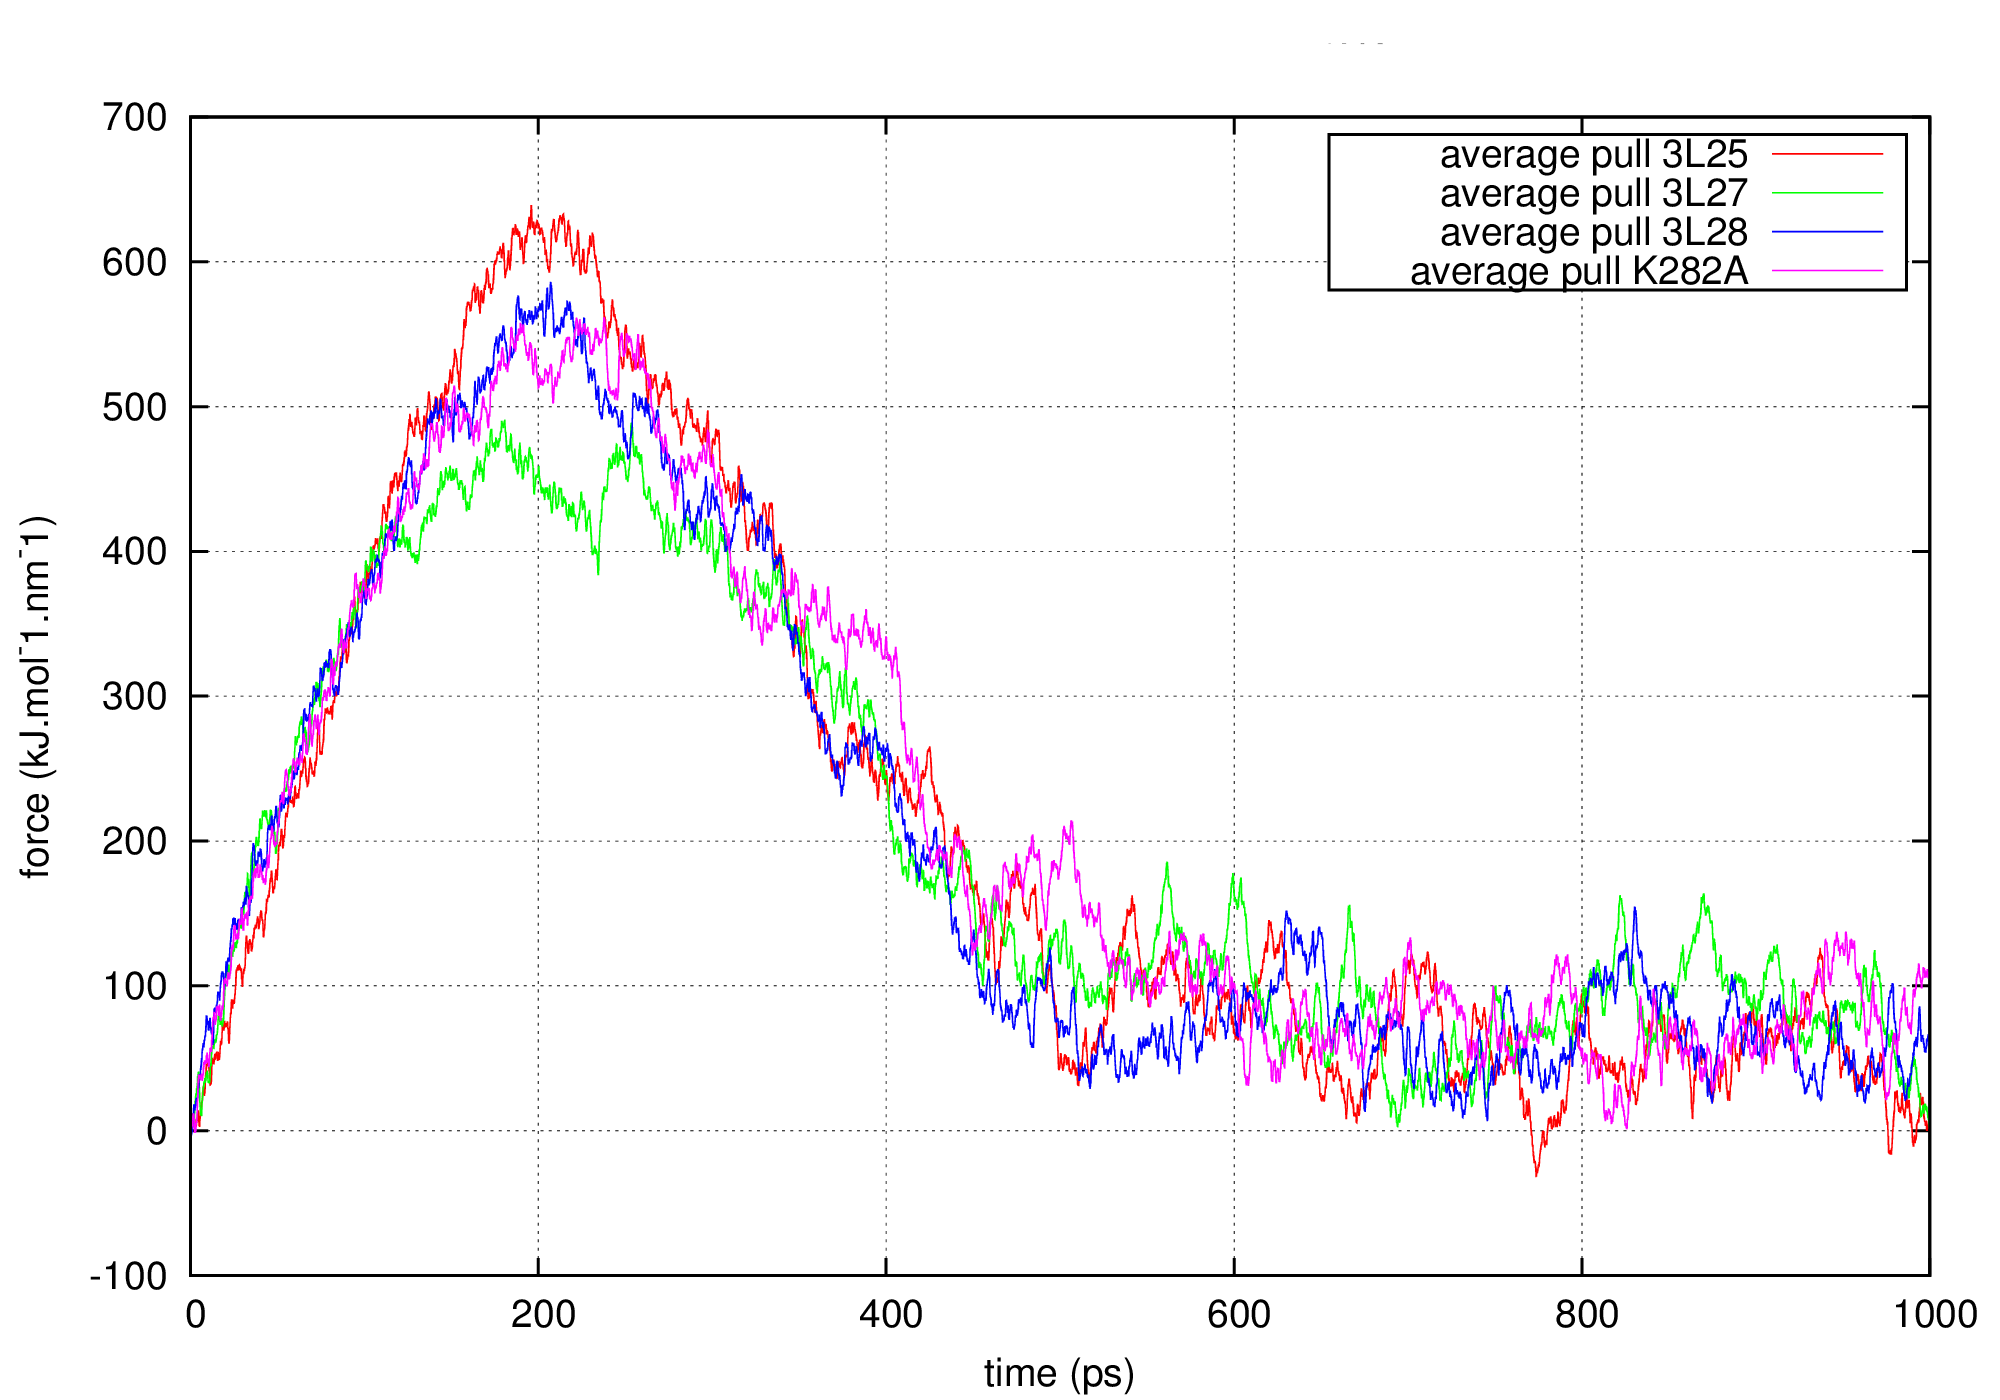
\includegraphics[width=0.95\textwidth,natwidth=610,natheight=642]{pullf}
	\caption{Đường biểu diễn lực kéo trung bình theo thời gian giữa dsRNA và VP35 với phân tử không đột biến (3L25) và đột biến (3L27, 3L28, \gls{K282A})}
	\label{pullft}
	\end{subfigure}
	\begin{subfigure}{0.95\textwidth}
	\centering
	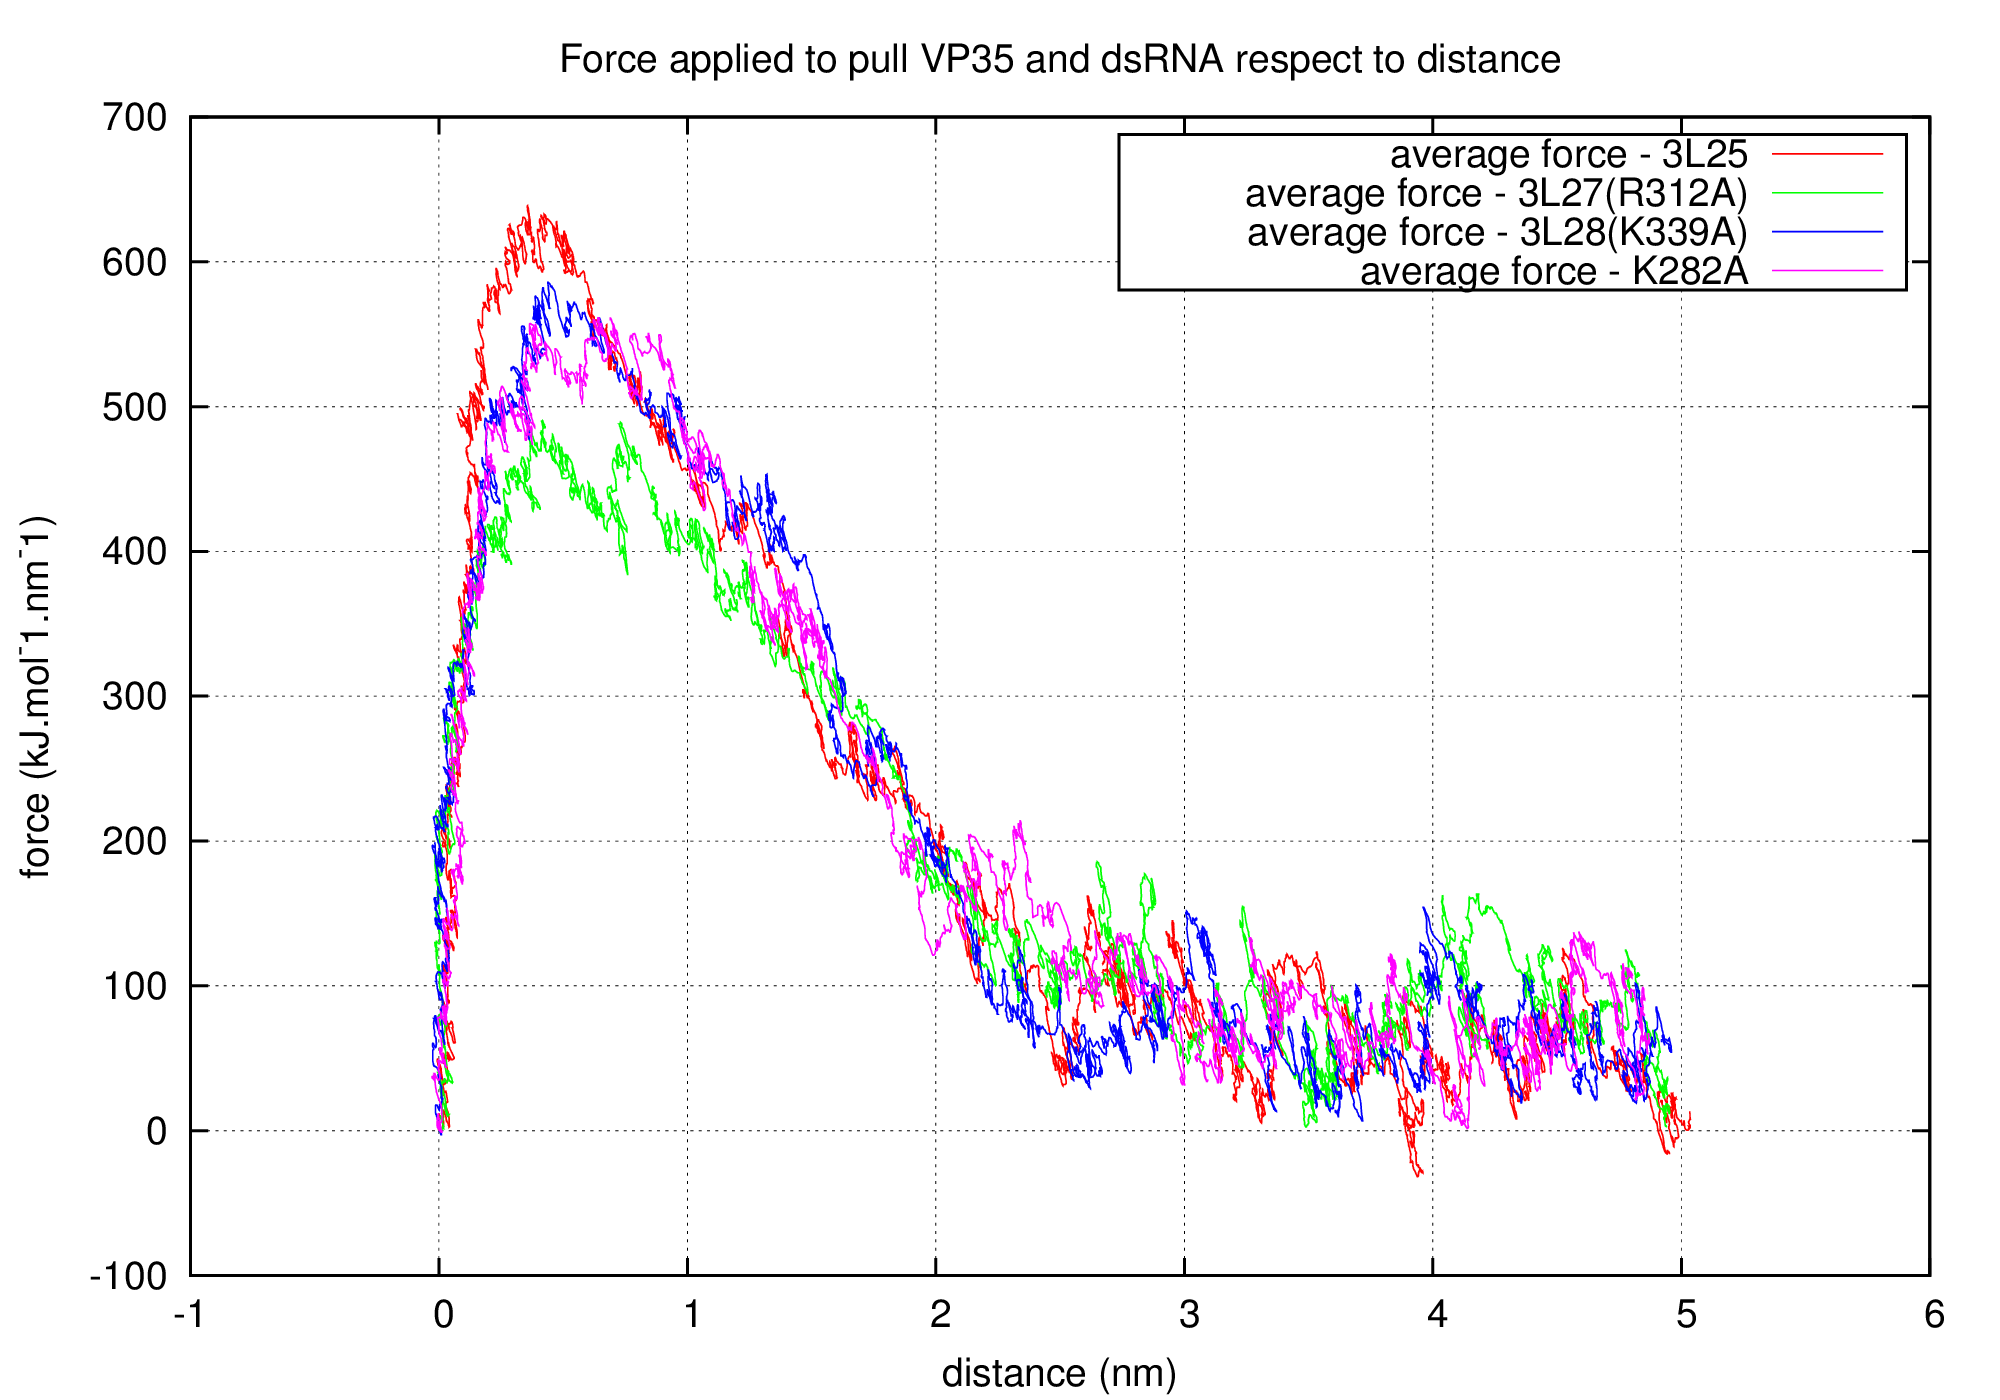
\includegraphics[width=0.95\textwidth,natwidth=610,natheight=642]{pullfx}
	\caption{Đường biểu diễn lực kéo trung bình theo toạ độ khối tâm của dsRNA của phân tử không đột biến (3L25) và đột biến (3L27, 3L28, \gls{K282A})}
	\label{pullfx}
	\end{subfigure}
	\label{}
	\end{figure}

Tương tự với cấu hình 3L28 (đột biến amino acid 339 từ Lysine sang Alanine - \gls{K339A}), lực kéo tối đa dùng để tách hai nhóm phân tử thấp hơn so với lực kéo trong quá trình mô phỏng phân tử gốc 3L25, điều này phù hợp với kết quả thực nghiệm\cite{Leung2010}.
\section{Đột biến Lys282Ala}
Từ dữ liệu thu được trong quá trình mô phỏng các cấu hình không đột biến và đột biến, đề tài phát triển thêm một bước ở việc dự đoán amino acid Arginine thứ 282 cũng đóng vai trò quan trọng trong tương tác dsRNA-VP35 dựa trên các quan sát sau:
\begin{itemize}
\item Lys282 là phân tử Arginine mang điện tích, vì vậy nó có thể đóng góp cho tương tác giữa hai nhóm phân tử trong tương tác tĩnh điện. Hơn nữa, kết quả phân tích thế năng cho thấy Lys282 đóng góp nhiều vào tương tác \gls{dsrna}--VP35 (xem hình \ref{fig:282}). Độ thay đổi thế năng tương tác giữa Lys282 với \gls{dsrna} (trên $140kJ/mol$) lớn hơn so với độ thay đổi thế năng tương tác giữa Arg312 với \gls{dsrna} (khoảng $140kJ/mol$). Thực nghiệm cho thấy đột biến Arg312Ala làm mất hoàn toàn khả năng gắn vào \gls{dsrna} của VP35.
\item Lys282 là một trong những amino acid tạo liên kết Hydro mạnh trong cả 3 lần mô phỏng \gls{smd} (xem hình \ref{fig:hbond3L25_pull1},\ref{fig:hbond3L25_pull2},\ref{fig:hbond3L25_pull3}). Cụ thể, Lys282 luôn tạo liên kết Hydro ở mức 100\% trong suốt thời gian VP35 vẫn còn tương tác với \gls{dsrna}.
\end{itemize}
Để đánh giá kết quả tiên đoán, đường biểu diễn lực kéo trung bình cấu hình đột biến Lys282 cho thấy lực kéo tối đa của phân tử này thấp hơn so với phân tử không đột biến và tương đối xấp xỉ với lực kéo tối đa cho cấu hình đột biến 3L28 (đột biến Lys339Ala) có được từ thực nghiệm. Như vậy, Lys282 có thể là một trong những amino acid chính đóng góp vào tương tác dsRNA-VP35. Việc đột biến phân tử này gây ảnh hưởng lên tương tác dsRNA-VP35 một cách rõ rệt.
%	\begin{figure}[t]
%	\centering
%	\includegraphics[height=0.3\textheight,natwidth=610,natheight=642]{../../../Analysis/non_md/3L25/hbond}
%	\caption{Tỉ lệ \% liên kết hydro tạo bởi các cặp amino acid và \gls{dsrna}}
%	\label{fig:hbond25}
%	\end{figure}
%	\begin{figure}[p]
%	\centering
%	\includegraphics[height=0.3\textheight,natwidth=610,natheight=642]{../../../Analysis/non_md/3L27/hbond}
%	\caption{Tỉ lệ \% liên kết hydro tạo bởi các cặp amino acid và \gls{dsrna}}
%	\label{fig:hbond27}
%	\end{figure}
%	\begin{figure}[p]
%	\centering
%	\includegraphics[height=0.3\textheight,natwidth=610,natheight=642]{../../../Analysis/non_md/3L28/hbond}
%	\caption{Tỉ lệ \% liên kết hydro tạo bởi các cặp amino acid và \gls{dsrna}}
%	\label{fig:hbond28}
%	\end{figure}
%	\subsection{Phân tử không đột biến}
%
%	Dựa vào đồ thị lực kéo dùng để tách VP35 khỏi \gls{dsrna} theo thời gian dễ dàng xác định được giá trị lực kéo tối đa. Lực kéo tối đa này cho thấy VP35 chuỗi B gắn khá chặt vào \gls{dsrna} 
%	\subsection{Đột biến Arg312Ala}
%
%	\subsection{Đột biến Lys339Ala}
%
%\section{AB-conf}
%
%%%%%%%%%%%%%%%%%%%%%%%%%%%%%%%%%%%%%%%%%%%
%+ Ket thuc Chuong 3.
%%%%%%%%%%%%%%%%%%%%%%%%%%%%%%%%%%%%%%%%%%%


\newpage
\pagestyle{fancy}
%%%%%%%%%%%%%%%%%%%     Chuong 4       %%%%%%%%%%%%%%%%%%%%%%%%
%%%%%%%%%%%%%%%%%%%                    %%%%%%%%%%%%%%%%%%%%%%%%
\setcounter{chapter}{3}
\chapter{Kết luận và hướng phát triển tiếp theo của đề tài}

	
	
	Khóa luận được thực hiện trong thời gian ngắn và đạt được những kết quả về vai trò của các amino acid Arg312 và Lys339 phù hợp với kết quả trong thực nghiệm, đồng thời dự đoán amino acid đóng góp vào tương tác giữa dsRNA-VP35.

	Kết quả thu được từ khóa luận đem lại gợi ý cho việc phát triển các phân tử có thể tác động vào các amino acid đóng góp vào tương tác dsRNA--VP35. Đồng thời gợi ý amino acid Lys282 đóng vai trò quan trọng trong tương tác \gls{dsrna}--VP35.
	
	Tuy nhiên, đề tài cần được thực hiện thêm quá trình mô phỏng động học thời gian dài để quan sát các trạng thái khác nhau của hệ phân tử, qua đó đánh giá chính xác hơn các amino acid đóng góp chủ yếu cho tương tác dsRNA--VP35.
	
	Hướng phát triển tiếp theo của đề tài sẽ là:
	\begin{itemize}
	\item Khảo sát phân tử VP35 đột biến Arg322Ala để kiểm tra giả thiết ở phần \ref{potential} và \ref{hbond-result}.
	\item Tiên đoán các phân tử có khả năng gắn vào khu vực tương tác dsRNA-VP35, theo đó gợi ý phân tử thuốc có khả năng bất hoạt VP35.
	\item Đánh giá và tiên đoán dựa trên mô phỏng động học phân tử thời gian dài nhằm tìm ra các amino acid đóng góp cho tương tác dsRNA-VP35.
	\end{itemize}
	
%%%%%%%%%%%%%%%%%%%%%%%%%%%%%%%%%%%%%%%%%%%
%+ Ket thuc Chuong 4.
%%%%%%%%%%%%%%%%%%%%%%%%%%%%%%%%%%%%%%%%%%%


%%%%%%%%%%%%%%%%%%%     Bibliography    %%%%%%%%%%%%%%%%%%%%%%%
%%%%%%%%%%%%%%%%%%%                     %%%%%%%%%%%%%%%%%%%%%%%
%\nocite{*}
\printbibliography
\addcontentsline{toc}{chapter}{Tài liệu tham khảo}
\clearpage





%%%%%%%%%%%%%%%%%%%     Appendice       %%%%%%%%%%%%%%%%%%%%%%%
%%%%%%%%%%%%%%%%%%%                     %%%%%%%%%%%%%%%%%%%%%%%
\appendix
\addcontentsline{chapter}{Phụ lục}
\clearpage
\newpage
\chapter{Các amino acid tương tác với \glsentrytext{dsrna}}
\label{81residues}
\begin{multicols}{3}
\begin{tabular}{l|c c}
\hline
STT & Vị trí & Tên \\
\hline
1 & 228& Met \\
2 & 229& Tyr \\
3 & 230& Asp \\
4 & 231& His \\
5 & 232& Leu \\
6 & 233& Pro \\
7 & 234& Gly \\
8 & 235& Phe \\
9 & 236& Gly \\
10 & 237& Thr \\
11 & 238& Ala \\
12 & 239& Phe \\
13 & 240& His \\
14 & 241& Gln \\
15 & 242& Leu \\
16 & 243& Val \\
\end{tabular}

\begin{tabular}{l|c c}
\hline
STT & Vị trí & Tên \\
\hline
17 & 246& Ile \\
18 & 259& Ile \\
19 & 261& Ala \\
20 & 262& Glu \\
21 & 263& Phe \\
22 & 264& Gln \\
23 & 265& Ala \\
24 & 266& Ser \\
25 & 267& Leu \\
26 & 268& Ala \\
27 & 269& Glu \\
28 & 270& Gly \\
29 & 271& Asp \\
30 & 272& Ser \\
31 & 273& Pro \\
32 & 274& Gln \\
\end{tabular}

\begin{tabular}{l|c c}
\hline
STT & Vị trí & Tên \\
\hline
33 & 275& Cys \\
34 & 276& Ala \\
35 & 277& Leu \\
36 & 278& Ile \\
37 & 279& Gln \\
38 & 280& Ile \\
39 & 281& Thr \\
40 & 282& Lys \\
41 & 283& Arg \\
42 & 284& Val \\
43 & 285& Pro \\
44 & 287& Phe \\
45 & 288& Gln \\
46 & 289& Asp \\
47 & 290& Ala \\
48 & 292& Pro \\
\end{tabular}

\begin{tabular}{l|c c}
\hline
STT & Vị trí & Tên \\
\hline
49 & 300& Arg \\
50 & 301& Gly \\
51 & 303& Ile \\
52 & 304& Pro \\
53 & 305& Arg \\
54 & 306& Ala \\
55 & 307& Cys \\
56 & 308& Gln \\
57 & 309& Lys \\
58 & 310& Ser \\
59 & 311& Leu \\
60 & 312& Arg \\
61 & 313& Pro \\
62 & 314& Val \\
63 & 315& Pro \\
64 & 316& Pro \\
\end{tabular}

\begin{tabular}{l|c c}
\hline
STT & Vị trí & Tên \\
\hline
65 & 317& Ser \\
66 & 318& Pro \\
67 & 319& Lys \\
68 & 320& Ile \\
69 & 321& Asp \\
70 & 322& Arg \\
71 & 323& Gly \\
72 & 324& Trp \\
73 & 325& Val \\
74 & 326& Cys \\
75 & 328& Phe \\
76 & 335& Thr \\
77 & 336& Leu \\
78 & 337& Gly \\
79 & 338& Leu \\
80 & 339& Lys \\
\end{tabular}

\begin{tabular}{l|c c}
\hline
STT & Vị trí & Tên \\
\hline
81 & 340 & Ile \\
\end{tabular}
\end{multicols}

\newpage
\chapter{Khảo sát liên kết Hydro}
\label{hbond}
\begin{figure}[h!]
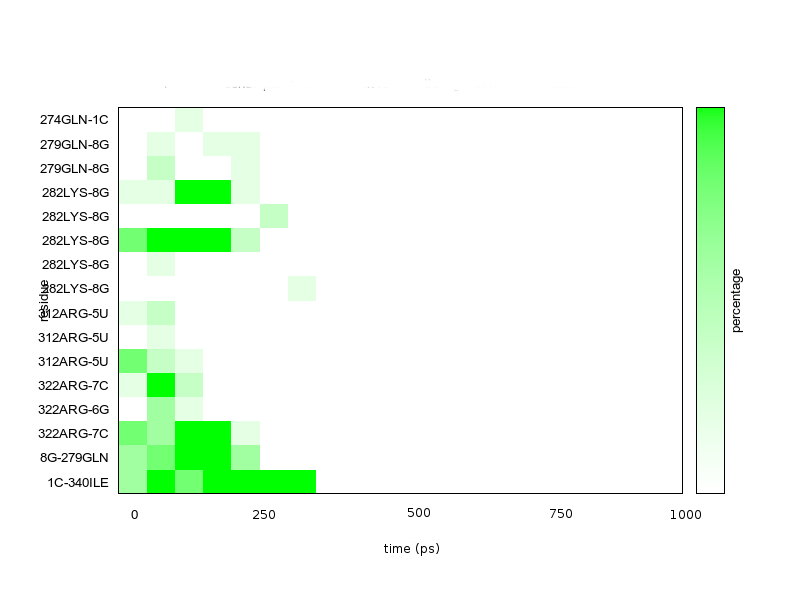
\includegraphics[width=\textwidth,natwidth=610,natheight=642]{hbond3L25_pull1}
%\vspace{-40pt}
\caption{Liên kết Hydro theo thời gian giữa các \gls{residue} và \gls{dsrna}. Lần kéo thứ 1 cấu hình B-conf phân tử có PDBID: 3L25}
\label{fig:hbond3L25_pull1}
\end{figure}
\begin{figure}[h!]
%\vspace{-20pt}
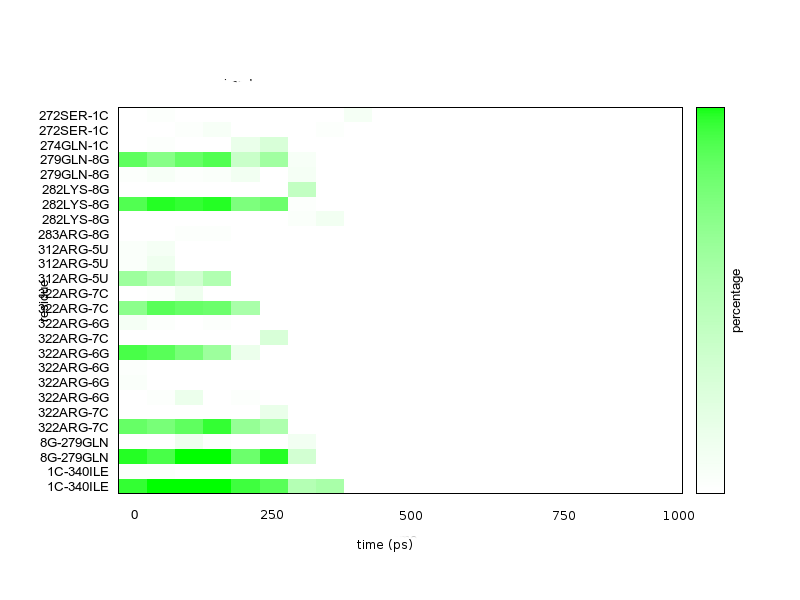
\includegraphics[width=\textwidth,natwidth=610,natheight=642]{hbond3L25_pull3}
%\vspace{-40pt}
\caption{Liên kết Hydro theo thời gian giữa các \gls{residue} và \gls{dsrna}. Lần kéo thứ 3 cấu hình B-conf phân tử có PDBID: 3L25}
\label{fig:hbond3L25_pull3}
\end{figure}
%\newpage
\chapter{Các amino acid và các ký hiệu tương ứng}
\begin{multicols}{2}
\begin{tabular}{l|c c}
\hline
Tên đầy đủ & 3 ký tự & 1 ký tự \\
\hline
Alanine & ALA & A \\
Cysteine & CYS & C \\
Aspartic acid & ASP & D \\
Glutamic acid & GLU & E \\
Phenylalanine & PHE & F \\
Glycine & GLY & G \\
Histidine & HIS & H \\
Isoleucine & ILE & I \\
Lysine & LYS & K \\
Leucine & LEU & L \\
\end{tabular}

\begin{tabular}{l|c c}
\hline
Tên đầy đủ & 3 ký tự & 1 ký tự \\
\hline
Methionine & MET & M \\
Asparagine & ASN & N \\
Proline & PRO & P \\
Glutamine & GLN & Q \\
Arginine & ARG & R \\
Serine & SER & S \\
Threonine & THR & T \\
Valine & VAL & V \\
Tryptophan & TRP & W \\
Tyrosine & TYR & Y \\
\end{tabular}
\end{multicols}
\end{document}
